%% =====================================================================
%% main-llmxive.tex — content-extracted llmXive wrapper
%% =====================================================================
%% Generated by scripts/extract_paper_content.py. The original paper
%% body is preserved; the venue-specific preamble (class, bundled .cls
%% files, custom packages) is DISCARDED and replaced with the llmxive
%% house style + a shim block that no-ops any venue-specific macros the
%% body still references.
%% =====================================================================
\documentclass{llmxive}


%% ── Packages forwarded from original preamble ─────────────────
\usepackage[toc,page,header]{appendix}
\usepackage{url}
\usepackage{wrapfig}
\usepackage{tabularx}
\usepackage{enumitem}
\usepackage{listings}
\usepackage{amsfonts}
\usepackage{amsmath}
\usepackage{etoolbox}
\usepackage{lipsum}
\usepackage{xspace}
\usepackage{fontawesome5}
\usepackage{placeins}
\usepackage{hyphenat}
\usepackage{parskip}
\usepackage{ulem}
\usepackage{graphicx}
\usepackage{subcaption}
\usepackage{multirow}
\usepackage{bm}
\usepackage[most]{tcolorbox}
\usepackage[noabbrev,nameinlink]{cleveref}
\usepackage{natbib}

%% ── Shim layer (venue macros made into no-ops) ────────────────
\makeatletter
\providecommand{\TODO}[1]{}
\providecommand{\acknowledgments}{\section*{Acknowledgments}}
\providecommand{\address}[1]{}
\providecommand{\affiliation}[1]{}
\providecommand{\aistatsfinalcopy}{}
\providecommand{\animategraphics}[5][]{\includegraphics[#1]{#3#4}}
\providecommand{\argmax}{\mathop{\mathrm{arg\,max}}}
\providecommand{\argmin}{\mathop{\mathrm{arg\,min}}}
\providecommand{\authorrunning}[1]{}
\providecommand{\blfootnote}[1]{\footnote{#1}}
\providecommand{\corresponding}{}
\providecommand{\correspondingauthor}[1]{}
\providecommand{\eg}{e.g.,\xspace}
\providecommand{\email}[1]{\href{mailto:#1}{#1}}
\providecommand{\equalcontribution}{}
\providecommand{\etal}{et al.\xspace}
\providecommand{\etc}{etc.\xspace}
\providecommand{\iclrfinalcopy}{}
\providecommand{\icmlfinalcopy}{}
\providecommand{\ie}{i.e.,\xspace}
\providecommand{\iid}{i.i.d.\xspace}
\providecommand{\institute}[1]{}
\providecommand{\keywords}[1]{\par\noindent\textbf{Keywords:} #1}
\providecommand{\neuripsfinalcopy}{}
\providecommand{\tablecite}[1]{\cite{#1}}
\providecommand{\titlerunning}[1]{}
\providecommand{\todo}[1]{}
\providecommand{\wrt}{w.r.t.\xspace}
\AtBeginDocument{\renewcommand{\and}{ \textperiodcentered\ }}
\makeatother

%% ── User-defined macros forwarded from original preamble ─────
\makeatletter
\providecommand{\faGlobe}{[Web]}
\providecommand{\faGithub}{[GH]}
\providecommand{\faEnvelope}{[Email]}
\providecommand{\faCalendar}{[Date]}
\providecommand{\faUsers}{[Authors]}
\providecommand{\ours}{\textsc{SkillsVote}\xspace}
\providecommand{\online}{\textsc{Online}\xspace}
\providecommand{\offline}{\textsc{Offline}\xspace}
\providecommand{\svgain}[1]{#1}
\providecommand{\svloss}[1]{#1}
\providecommand{\svup}[1]{$_{\svgain{\scriptstyle\uparrow #1}}$}
\providecommand{\svdown}[1]{$_{\svloss{\scriptstyle\downarrow #1}}$}
\providecommand{\bottomfraction}{0.75}
\providecommand{\textfraction}{0.10}
\providecommand{\arraystretch}{1.5}
\providecommand{\svpromptheading}[1]{\par\smallskip\noindent{\sffamily\bfseries#1}\par}
\providecommand{\svpromptsubheading}[1]{\par\smallskip\noindent{\sffamily\bfseries #1}\par}
\providecommand{\svinlinecode}[1]{{\ttfamily #1}}
\providecommand{\svpartsep}{\par\medskip\noindent{\leaders\hbox{\rule[0.45ex]{5pt}{0.35pt}\hspace{3pt}}\hfill\kern0pt}\par\medskip}
\providecommand{\svtrace}[2]{  \par\smallskip\noindent
  \begin{minipage}[t]{\svtracelabelwidth}#1\end{minipage}  \hspace{0.6em}  \begin{minipage}[t]{\dimexpr\linewidth-\svtracelabelwidth-0.6em\relax}#2\end{minipage}  \par
}
\providecommand{\svcasebenchmark}[1]{\par\noindent{\sffamily\scriptsize\bfseriesBenchmark: #1}\par\smallskip}
\providecommand{\beginappendix}{\appendix{\titlefont\sffamily \memblue{Appendix}\par}}
\definecolor{membg}{HTML}{5A7EFA}
\definecolor{memblue}{HTML}{5A7EFA}
\definecolor{memblue2}{HTML}{F0F8FF}
\newtcolorbox{svpromptbox}[1]{
  colback=memblue2,
  colframe=memblue,
  colbacktitle=memblue,
  coltitle=white,
  arc=1pt,
  boxrule=0.8pt,
  fonttitle=\bfseries\sffamily,
  fontupper=\small,
  title={#1},
  left=6pt,
  right=6pt,
  top=6pt,
  bottom=6pt,
  before skip=0.9em,
  after skip=1.0em,
  breakable,
  width=\linewidth
}
\makeatother

%% ── llmXive paper metadata ──────────────────────────────────
\title{\ours : Lifecycle Governance of Agent Skills from Collection, Recommendation to Evolution}
\author{Hongyi Liu \and Haoyan Yang \and Tao Jiang \and Bo Tang \and Feiyu Xiong \and Zhiyu Li}
\paperid{arXiv:2605.18401}
\paperstatus{Preprint}

\begin{document}
\maketitle
\begin{abstract}
Long-horizon LLM agents leave traces that could become reusable experience, but raw trajectories are noisy and hard to govern. We treat Agent Skills as an experience schema that couples executable scripts, with non-executable guidance on procedures. Yet open skill ecosystems contain redundant, uneven, environment-sensitive artifacts, and indiscriminate updates can pollute future context. We present \ours, a lifecycle-governance framework for Agent Skills from collection and recommendation to evolution. \ours profiles a million-scale open-source corpus for environment requirements, quality, and verifiability, then synthesizes tasks for verifiable skills. Before execution, \ours performs agentic library search over structured skill library to expose instructional skill context. After execution, it decomposes trajectories into skill-linked subtasks, attributes outcomes to skill use, agent exploration, environment, and result signals, and admits only successful reusable discoveries to evidence-gated updates. In our evaluation, \offline evolution improves GPT-5.2 on Terminal-Bench 2.0 by up to \svgain{7.9 pp}, while \online evolution improves SWE-Bench Pro by up to \svgain{2.6 pp}. Overall, governed external skill libraries can improve frozen agents without model updates when systems control exposure, credit, and preservation.
\end{abstract}
\par\noindent
\begin{minipage}{\linewidth}
  \centering
  \vspace{-5mm}
  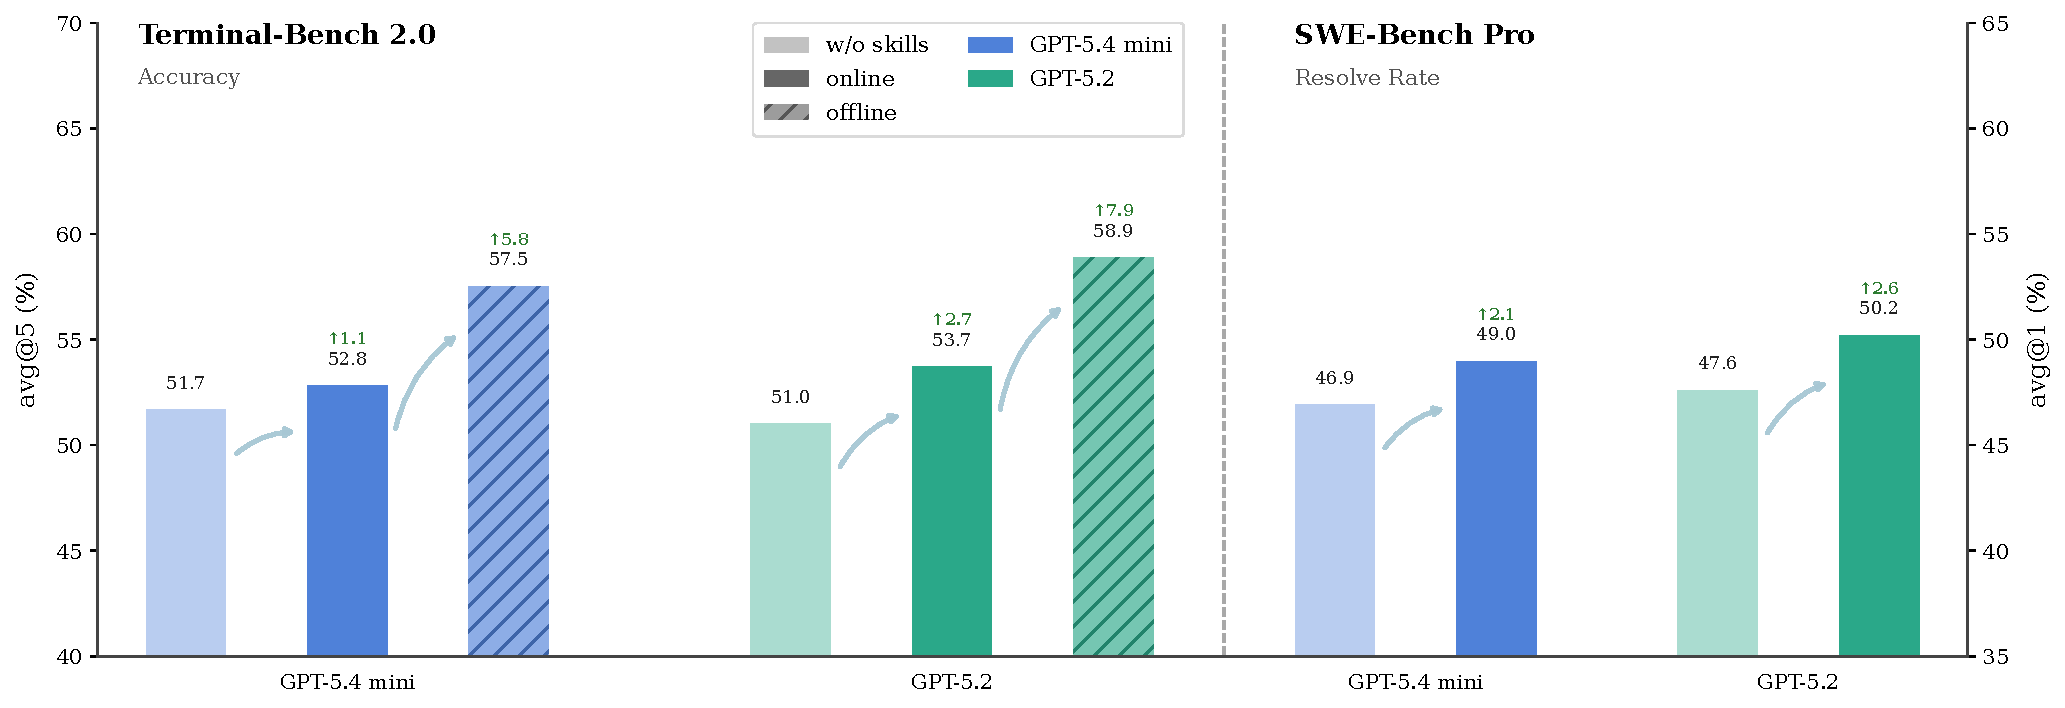
\includegraphics[width=0.98\linewidth]{assets/results_overview.pdf}
  \vspace{-2mm}
  \captionof{figure}{Main performance overview of \ours across Terminal-Bench 2.0 and SWE-Bench Pro.}
  \label{fig:results-overview}
\end{minipage}

\section{Introduction}
Recent progress in LLM agents has shifted the research focus from single-turn answer generation to systems that act over long horizons. Contemporary benchmarks require agents to repair realistic codebases \citep{jimenez2024swe,deng2025swe}, navigate web applications \citep{zhou2024webarena}, operate across desktop environments \citep{xie2024osworld}, and manipulate external state through APIs, tools, and terminals \citep{trivedi2024appworld,merrill2026terminal}. These settings produce trajectories that record intermediate decisions, tool interactions, and environmental feedback, not merely final answers. They also make experience reuse a first-order systems problem: each task yields operational evidence, but that evidence is distributed across low-level traces and must be selected before it can support future tasks. Prior work on experiential agents shows that such traces can be organized into reusable experience or skills that shape later behavior \citep{shinn2023reflexion,zhao2024expel,wang2024voyager}.

\begin{figure}[!b]
    \centering
    
\includegraphics[width=\linewidth]{assets/overview.pdf}
    \caption{\ours closes the Agent Skill lifecycle by coupling pre-task recommendation, in-task execution evidence, post-task attribution, and controlled library evolution. A profiled skill library is searched before execution to expose task-relevant skills; after execution, trajectories and outcome signals are decomposed into skill-linked subtasks so reusable successful explorations can edit existing skills or create new ones.}
    \label{fig:overview}
\end{figure}

Raw trajectories, however, are a weak substrate for long-term experience reuse. They are lengthy, noisy, tightly bound to local environments, and often conflate robust strategies with incidental state. Agent Skills provide a more structured schema for distilled experience: a skill can package procedural instructions, scripts, templates, references, dependency boundaries, and applicability conditions in a single artifact. This makes experience more compact than a full trajectory while preserving more executable context than an isolated natural-language summary \citep{jiang2026sok}.

At ecosystem scale, the problem is no longer only how to author an individual skill, but how to control a continuously expanding library. Public skill ecosystems already exhibit scale, redundancy, uneven quality, and safety risks \citep{ling2026agent}. Skill benchmarks further show that the benefit of skills depends on task, domain, and retrieval setting; weakly related or low-quality skills can degrade agent performance \citep{li2026skillsbench,liu2026well}. Treating skills as ecosystem artifacts also changes the failure mode: larger libraries increase coverage, but they also enlarge the search space and amplify library pollution when weakly supported lessons are incorporated indiscriminately. These observations suggest that large-scale skill ecosystems require collection, governance, profiling, recommendation, evaluation, and evolution to be treated as coupled processes \citep{li2026organizing,zheng2026skillrouter}. Against this background, \ours constructs and profiles a million-scale open-source Agent Skill corpus and governs how skills \textit{vote} into the agent context before execution and how attributed evidence \textit{votes} into the skill library after execution.

This paper introduces \ours, a lifecycle framework for Agent Skills. Before execution, \ours formulates recommendation as agentic search over a structured skill library rather than static semantic matching \citep{li2026beyond}. The recommender filters a small, relevant, and low-redundancy set of skills and supplies the agent with compressed usage context. After execution, \ours performs outcome attribution using the trajectory and visible result signal, explaining how the outcome relates to the selected skill, the agent's own exploration, environmental conditions, and the evaluation signal itself. These stages form the closed loop shown in Figure~\ref{fig:overview}.

This attribution layer addresses a specific gap in recent skill-evolution work. Existing systems demonstrate that execution evidence can improve skills by distilling local lessons from trajectory pools, aggregating multi-user sessions into shared skill updates, or diagnosing and revising domain skills from bad cases \citep{ni2026trace2skill,ma2026skillclaw,liu2026skillforge}. \ours uses this evidence under an attribution control layer: it first determines whether a success or failure is attributable to the selected skill, the agent's own exploration, the environment, or the result signal, and then constrains which experience may enter the evolving skill library. This control prevents spurious successes from being rewarded and keeps failures caused by the environment or evaluation signal from driving irrelevant repository edits. Thus, \ours connects recommendation, attribution, and controlled evolution into an auditable closed loop.

We evaluate \ours on Terminal-Bench 2.0 and SWE-Bench Pro \citep{merrill2026terminal,deng2025swe}. Our experiments study whether recommendation outperforms directly exposing the initial skill library, whether offline evolution builds a transferable cold-start library from historical tasks, and whether online evolution accumulates useful experience in a test-time task stream.

This paper makes the following contributions:
\begin{enumerate}
    \setlength{\itemsep}{0pt}
    \item We formulate an Agent Skill lifecycle framework that connects open-world collection and governance, recommendation, outcome attribution, and controlled evolution.
    \item We construct and profile a million-scale open-source Agent Skill corpus for systematic analysis and governance of open skill ecosystems.
    \item We design an attribution-guided recommendation-to-evolution loop that constrains skill library evolution and reduces the risk of indiscriminate library updates.
    \item We evaluate recommendation, offline transfer, and online evolution on terminal and software-engineering benchmarks with verifier-backed outcomes.
\end{enumerate}


% \section{Preliminary}
% % [llmxive-extract] missing input: sections/2_preliminary.tex


\section{Related Work}
\subsection{Evolution of Agent Experience Learning}
Agent experience learning has progressed from records reusable only in context to executable artifacts. Early memory methods store unstructured cases and examples, such as few-shot trajectories, exemplars, or human-curated interaction records \citep{zhou2025memento,zheng2024synapse,wang2026memgovern}. Workflow methods abstract traces into semi-structured workflows and SOPs \citep{wang2025agent,fang2025memp}, while strategy-level methods compress experience into principles, heuristics, and strategies \citep{zhao2024expel,ouyang2026reasoningbank,cao2025remember,zhang2026agentic,cai2025training,cai2025flex,wang2026procedural}. Recent tool, MCP, and skill-learning methods attach experience to callable interfaces, dependencies, and execution boundaries \citep{lu2026beyond,liu2025unifying,huang2025cascade}. Surveys and systems similarly frame memories, rules, skills, protocols, and harness components as deployment-time external artifacts \citep{zhang2026experience,zhou2026externalization,lin2026position,zhang2026autogenesis,liang2026genericagent,lin2026agentic}. \ours focuses on skill libraries: a skill combines procedural text, scripts, dependencies, and applicability boundaries, so experience remains auditable, versionable, and portable across harnesses, while full harness or protocol evolution has a larger action space.

\subsection{Agent Skill Ecosystems, Retrieval, and Evaluation}
As Agent Skills become installable and shareable file artifacts \citep{agentSkills,anthropic2026claudeCodeSkills,openai2026ChatgptSkillsDocs,skillsmp2026,skillssh2026,openclaw2026SkillsDocs,hermes2026AgentSkillsGuide,openclaw2026clawhub}, the problem shifts from authoring skills to governing and using open ecosystems. AgentSkillOS and SkillNet organize skills as ecosystem objects \citep{li2026organizing,liang2026skillnet}, while SkillsBench, SkillCraft, SkVM, and SkCC show that utility, compositional use, portability, security, dependencies, and harness compatibility must be evaluated before \texttt{SKILL.md} files can be trusted \citep{li2026skillsbench,chen2026skillcraft,skvm2026,ouyang2026skcc}. \ours profiles open-source skills for format, dependency, quality, and verifiability. At task time, governance does not remove selection: providing skills does not ensure correct selection, composition, or use. SkillRouter learns routing over full skill bodies rather than only names or descriptions \citep{zheng2026skillrouter}, while DCI replaces embedding retrieval with direct corpus interaction over source documents \citep{li2026beyond}. \ours lightly applies filesystem-native inspection to governed skill folders and outputs compact guidance for combining the selected skills.

\subsection{Skill-Centric Agent Self Evolution}
A growing body of work studies how agents learn and evolve around skill libraries. One line trains policies to decide when to retrieve a skill, how to use it, and when to distill behavior into the model or revise the library \citep{xia2026skillrl,wang2025reinforcement,xia2026metaclaw,wang2026openclaw,lu2026skill0,shi2026skill1,ouyang2026skillos}. Other systems keep the base model fixed and turn coarse session- or trajectory-level evidence, together with verifier or environment feedback, into reusable skill artifacts \citep{ni2026trace2skill,alzubi2026evoskill,zhang2026coevoskills,ma2026skillclaw,wang2026skillx,yang2026autoskill,si2026context,zhang2026skillflow,zhou2026memento,skillpro2026,gong2026skillmoo,xu2026multi}. \ours further factorizes each trajectory into judged, skill-linked subtasks, localizes the skill knowledge actually used and the responsibility for each outcome, and admits only reusable successful exploration into skill library evolution.


\section{Approach}
\ours treats Agent Skills as lifecycle artifacts. It first turns heterogeneous open-source skills into a profiled experience substrate, then controls which skills enter the solver agent context before execution and which execution evidence is allowed to update the library after execution.

\subsection{Open-Source Skill Corpus and Profiling}

\subsubsection{Collecting a Million-Scale Agent Skill Corpus}
Open Agent Skill ecosystems have already reached marketplace scale. SkillsMP and skills.sh aggregate \texttt{SKILL.md} packages from GitHub and expose search, categories, popularity, or installation-based discovery signals \citep{skillsmp2026,skillssh2026}. However, these discovery signals are insufficient for agent execution: a skill's name, description, or popularity does not establish whether it can run in the target environment, whether it describes a coherent capability, whether its referenced resources are complete, or whether its output can be objectively checked. Recent benchmarks likewise show that skill utility depends on the task, domain, and skill corpus quality \citep{li2026skillsbench,zhang2026skillflow}. \ours therefore builds a million-scale open-source corpus from GitHub \texttt{SKILL.md} files and treats each skill as a directory-level package rather than a text chunk. The required \texttt{SKILL.md} defines the capability and usage conditions, while optional \texttt{scripts/}, \texttt{references/}, and \texttt{assets/} directories preserve executable code, supporting documents, and templates.

\subsubsection{Profiling Skill Requirements, Quality, and Verifiability}
\ours profiles each skill along three dimensions. First, the runtime-requirement profile estimates operating-system assumptions, write permissions, \texttt{sudo} needs, network access, API keys, command-line tools, MCP servers, and environment variables. Second, the quality profile evaluates whether a skill is a stable execution unit through consistency, completeness, and task orientation. Third, the verifiability profile asks whether the skill has a low-ambiguity success condition, a reproducible sandbox environment, and task instances that can be constructed at reasonable cost. Prior ecosystem-level systems emphasize skill organization, multidimensional evaluation, and portability across model-harness combinations \citep{skvm2026,liang2026skillnet,li2026organizing}. \ours instantiates these concerns as execution-readiness profiles for open-source skills.

\subsubsection{Synthesizing Verifiable Tasks from Agent Skills}
For skills that pass the verifiability profile, \ours synthesizes tasks from the skill itself. Each task contains a clear instruction, a reproducible environment, and an executable verifier, following the Harbor task format \citep{harborFramework}. We then run real agent--model combinations on these tasks and record success rates, costs, execution traces, and verifier outcomes. This process links a static skill description to observed execution behavior. Not every skill is suitable for this step: preference-driven, open-world, or hardware-intensive skills remain profiled corpus items rather than forced benchmark tasks.

\subsection{Skill Recommendation via Agentic Library Search}

Existing skill harnesses commonly rely on progressive disclosure: the solver agent first sees lightweight skill metadata, and the full \texttt{SKILL.md} and supporting resources are loaded only after the skill appears relevant \citep{openai2026codexSkills,anthropic2026claudeCodeSkills,agentSkills}. This design lets many skills coexist in one environment, but it also compresses pre-task selection into short descriptions and limited path cues. SkillRouter further shows that, in large skill pools, the full skill body often carries decisive routing signals \citep{zheng2026skillrouter}. \ours builds on this progressive-disclosure interface by adding a task-conditioned exposure-control layer before the solver agent starts execution.

The motivation extends beyond skill systems. Filesystem-native atomic tools are increasingly used as a general interface for agentic search: DCI lets agents interact directly with corpora in deep-research-style retrieval rather than consuming a fixed top-$k$ interface \citep{li2026beyond}; code-search systems such as CodeScout and SWE-grep train multi-turn localization over ordinary repository tools \citep{sutawika2026codescout,pan2025swegrep}; Vercel's data-agent studies compress query exploration and validation into a small set of file and shell operations \citep{qu2025we,goyal2026testing}; and Letta uses a filesystem backend for agent-memory retrieval \citep{letta2025benchmarking}. These examples motivate treating an evolving skill library as a searchable file-based substrate.

Given a task and a profiled skill library, \ours runs a separate recommendation stage. The agent does not solve the task. It searches the local skill library, selectively reads candidate \texttt{SKILL.md} files and related resources, and selects skills that cover the task, fit the target environment, and provide complementary guidance. The output is a compact set of exposed skills plus a short usage guide for the solver agent, rather than the full library, a metadata-only routing decision, or a single-step top-$k$ chunk list. The recommendation record also anchors later attribution: after execution, \ours can inspect whether exposed skills were actually used and whether they contributed reusable discoveries.

\subsection{Distilling Execution Traces into Evolvable Units}
Recent work exposes a granularity gap in learning from agent execution. Agent evaluation commonly relies on task-level success signals, which are authoritative but provide sparse supervision for long-horizon tool use and make credit assignment difficult \citep{fan2026agentprocessbench}. Meanwhile, skill-learning systems show that execution trajectories contain reusable experience that can improve future behavior \citep{ni2026trace2skill,fang2026trajectory}. However, these works also suggest that trajectories must be filtered before they become reusable artifacts: a run may mix skill-guided actions, independent exploration, corrected failures, and redundant operational steps. At the other end, process-level benchmarks and failure-diagnosis methods annotate individual agent steps, showing the value of local feedback for analysis \citep{fan2026agentprocessbench,barke2026agentrx}. However, a single tool call rarely constitutes reusable skill knowledge. As shown in Figure~\ref{fig:attribution-granularity}, skill evolution thus requires an intermediate unit between full trajectories and individual steps.

\begin{figure}[t]
    \centering
    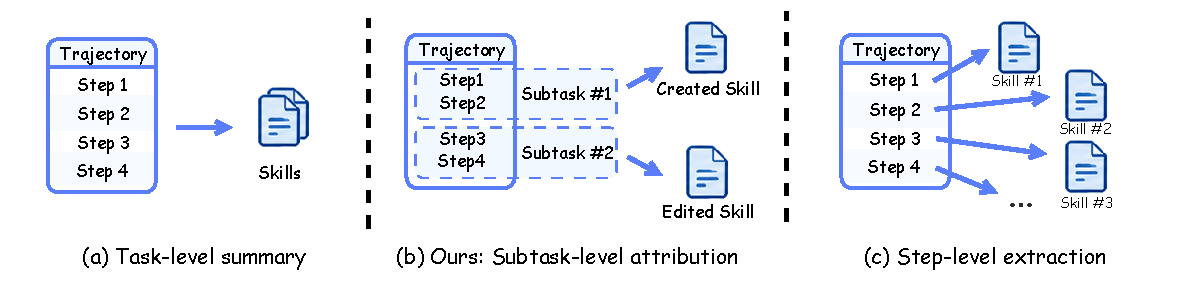
\includegraphics[width=\linewidth]{assets/method_contrast.pdf}
    \caption{Attribution granularity determines whether trajectory evidence can support skill evolution. Task-level summaries are too coarse for credit assignment, while step-level extraction is too fragmented; \ours uses subtask-level attribution to connect coherent execution segments to skill updates.}
    \label{fig:attribution-granularity}
\end{figure}

\ours addresses this mismatch by inserting a subtask-level attribution layer between full trajectories and individual tool calls. \textbf{A subtask is the smallest semantically complete unit that can support library evolution}: it has \textit{one standalone objective}, \textit{one primary evaluation signal}, and \textit{at most one associated skill context}. The primary evaluation signal specifies what kind of evidence can support the subtask outcome, such as environment feedback, human review, or no explicit signal. Trajectories are split only when one of these three boundaries changes, rather than whenever the agent issues another command. This granularity is local enough to assign responsibility, yet abstract enough to capture reusable procedures, constraints, and recovery patterns.

For each subtask, attribution compresses the execution evidence along three axes:

\begin{enumerate}
    \item \textbf{Outcome evidence.} The system records whether the subtask can be assessed by objective environment feedback, depends on human preference, or lacks an explicit evaluation signal. This prevents verifier-backed outcomes, subjective goals, and unsupported claims from being treated alike.
    \item \textbf{Responsibility assignment.} The system assigns both the final state and its main cause. Successful subtasks may be credited to skill-guided execution, independent exploration, or exploration after observing an irrelevant skill. Failed or uncertain subtasks are retained as diagnostic evidence, but they do not directly authorize skill evolution.
    \item \textbf{Reusable delta.} For skill-related subtasks, the system localizes the portions of skill knowledge that actually shaped execution, rather than crediting every exposed skill. It also extracts only reusable discoveries, such as missing procedures, preconditions, or recovery patterns, while discarding ordinary trial-and-error, task-specific constants, and repetitive operational details.
\end{enumerate}

\begin{figure}[t]
    \centering
    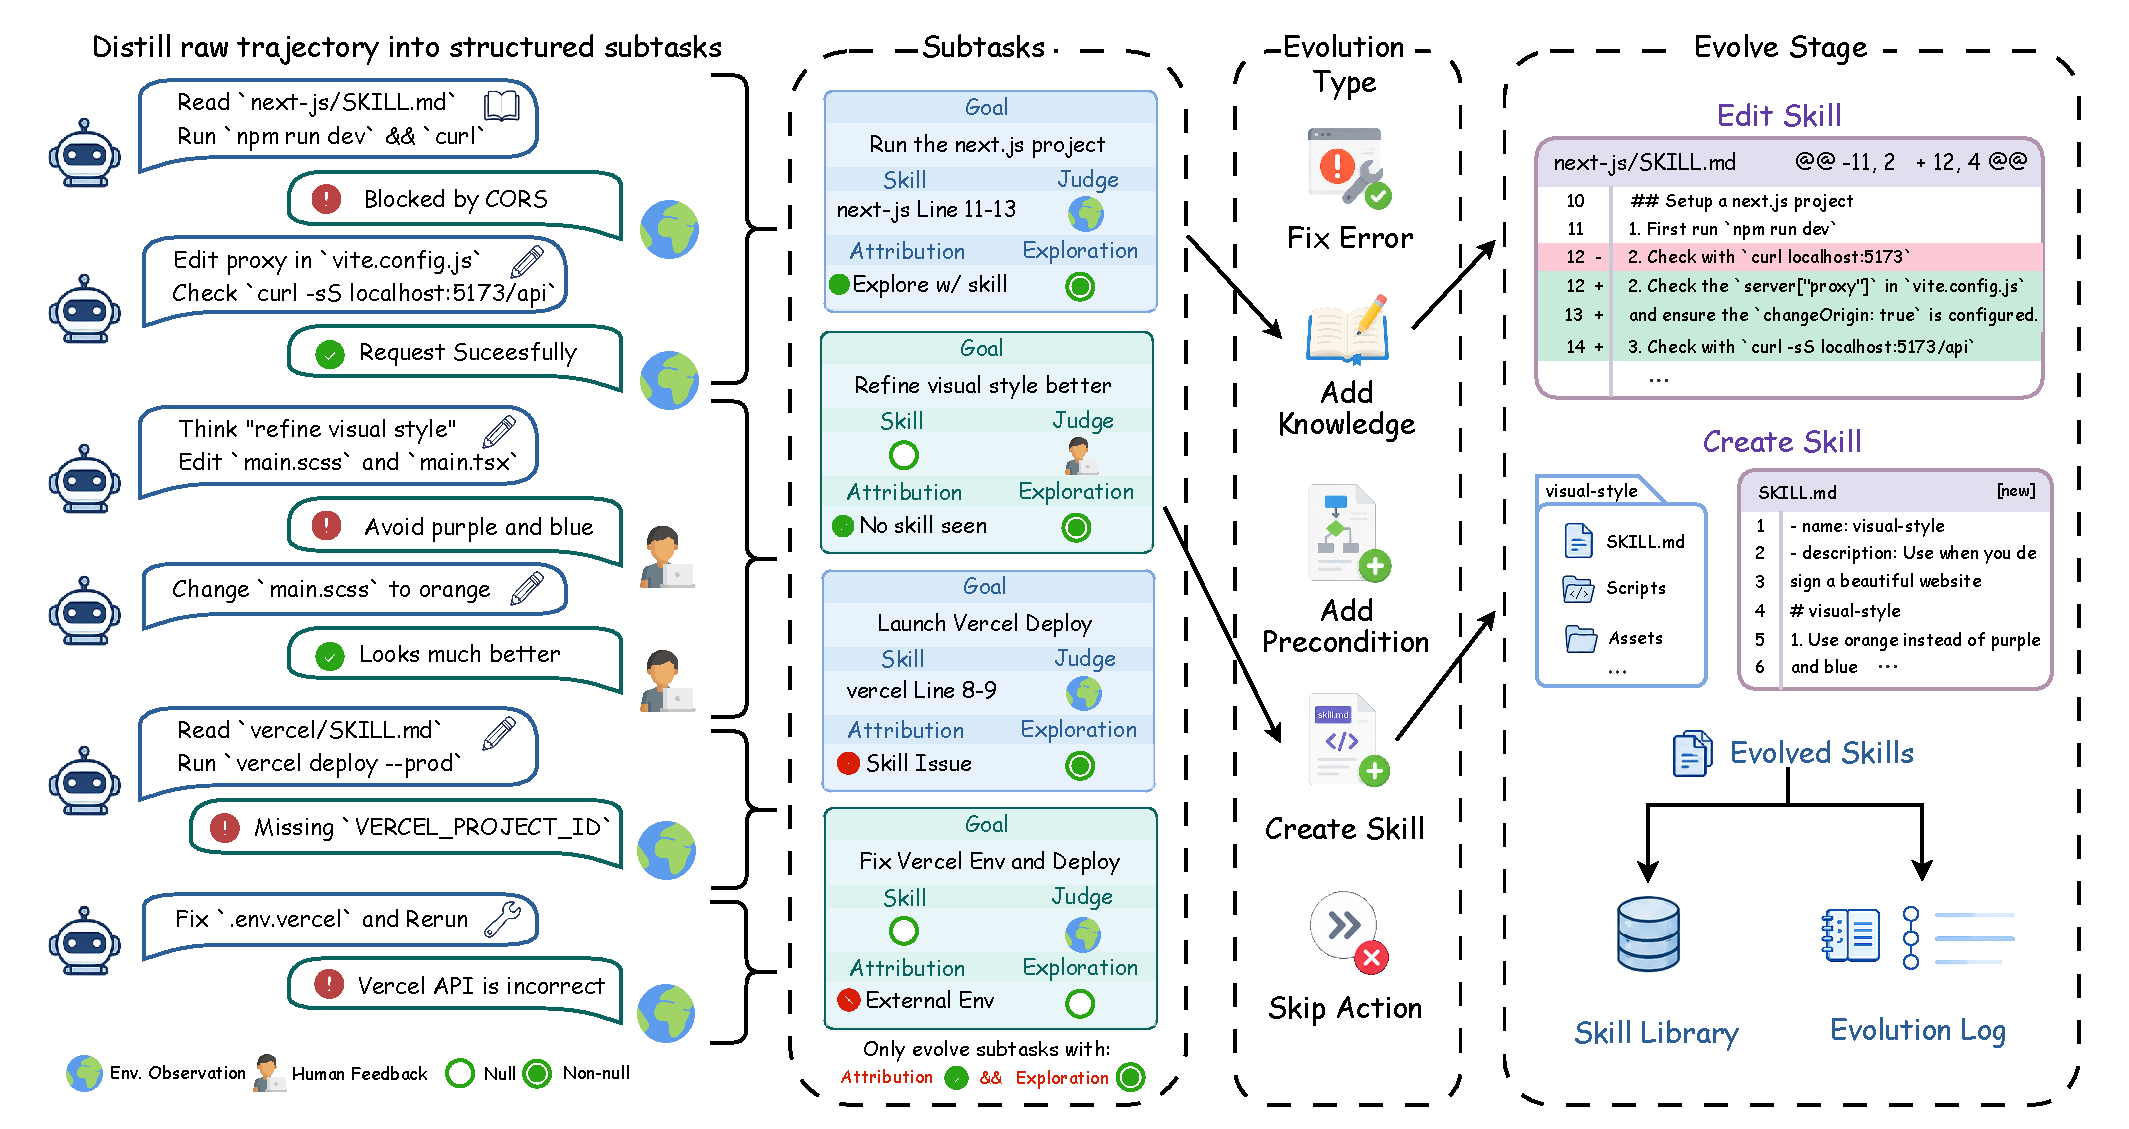
\includegraphics[width=\linewidth]{assets/attribution_evolve_pipeline.pdf}
    \caption{\ours distills raw execution traces into evidence-bound evolvable units and routes them to conservative library updates. Only successful subtasks that pass the attribution and reusable-exploration gates can trigger skill edits or new skill creation; external-environment outcomes and other non-admissible units are skipped.}
    \label{fig:attribution-pipeline}
\end{figure}

Together, these fields define an evolvable unit for the trajectory evidence in Figure~\ref{fig:attribution-pipeline}: evidence-bound, responsibility-aware, and reusable. These units form the interface to controlled evolution, where only successful subtasks with reusable exploration can propose library updates.

\subsection{Evidence-Based Controlled Skill Evolution}

The attribution layer produces evolvable units, but library evolution still requires explicit control over what evidence is allowed to change persistent skills. \ours formulates this step as evidence-gated update construction with explicit admissibility, aggregation, and routing criteria.

\paragraph{Admissibility.} \ours first filters which units may trigger evolution. A unit is admissible only if it is successful and contains reusable exploration. Failed, uncertain, or weakly supported evidence may remain useful for diagnosis, but it cannot directly authorize a skill update.
\paragraph{Aggregation.} Admissible units are then grouped before any edit is made. Units that support the same reusable procedure, precondition, workaround, or correction are merged into a single proposed update, so repeated observations strengthen one change rather than producing duplicate or fragmented edits.
\paragraph{Routing.} Finally, \ours routes each aggregated evidence group to an update action. If the evidence extends a skill that actually shaped execution, the system edits that skill through the smallest justified change: fixing incorrect guidance, adding missing knowledge, or tightening prerequisites. If the evidence reflects an independent reusable capability outside the current skill boundary, the system creates a new skill. When evidence is weak, redundant, or semantically misaligned with the target skill, it skips evolution.

Thus, skill evolution is conservative by design: every library change must be supported by attributed execution evidence, localized to the relevant skill boundary, and expressed as reusable procedural knowledge rather than a trajectory recap.


\section{Experiments}
\subsection{Experimental Setup}
We organize the evaluation around three questions that correspond to the main control points in the \ours lifecycle:
\begin{enumerate}
    \item \textbf{Offline evolution.} Can historical trajectories be distilled into a cold-start skill library that transfers to unseen tasks?
    \item \textbf{Online evolution.} Can the library accumulate useful experience over a sequential task stream?
    \item \textbf{Recommendation.} Given a skill library, does task-conditioned recommendation outperform exposing the library wholesale?
\end{enumerate}

\paragraph{Benchmarks.}
We evaluate \ours with Harbor on Terminal-Bench 2.0 and SWE-Bench Pro public \citep{harborFramework,merrill2026terminal,deng2025swe}. Terminal-Bench 2.0 contains 89 difficult terminal tasks inspired by real workflows; SWE-Bench Pro public contains 731 long-horizon software-engineering tasks from 11 public repositories. Following the leaderboards, we report avg@5 Accuracy and avg@1 Resolve Rate, respectively, ordering SWE-Bench Pro tasks by repository. Terminal-Bench Pro supplies offline data: we retain 48 public software-engineering and system-administration tasks, excluding 2 environment-unstable tasks \citep{wang2025let}.

\paragraph{Configurations.}
All settings use Codex with \texttt{GPT-5.2} or \texttt{GPT-5.4 mini} \citep{openai2025gpt52,openai2026gpt54MiniNano}. Both benchmarks include a no-skill baseline and an online setting that starts empty and evolves with task-level recommendation. Terminal-Bench 2.0 also includes an offline setting: a library is first built from 48 Terminal-Bench Pro historical tasks, with evolution triggered after every 4 tasks; the frozen library is then transferred to Terminal-Bench 2.0 for recommendation only.

\subsection{Main Results}
Tables~\ref{tab:main-results-tb2} and~\ref{tab:main-results-swebenchpro} report the main performance. On Terminal-Bench 2.0, \ours improves Accuracy in both offline and online settings. Offline evolution gives the clearest signal: a frozen library distilled from 48 Terminal-Bench Pro trajectories transfers to unseen tasks, improving GPT-5.2 by \svgain{+7.9 pp} and GPT-5.4 mini by \svgain{+5.8 pp}. This suggests that trajectory-derived skills can form a useful cold-start library rather than merely capturing source-task artifacts.

Online evolution yields smaller but positive gains. Starting from an empty library, \ours improves Terminal-Bench 2.0 Accuracy by \svgain{+2.7 pp} with GPT-5.2 and \svgain{+1.1 pp} with GPT-5.4 mini. On SWE-Bench Pro, online evolution improves Resolve Rate for both backbones: GPT-5.2 rises from 47.6 to 50.2, a \svgain{+2.6 pp} gain, and GPT-5.4 mini rises from 46.9 to 49.0, a \svgain{+2.1 pp} gain. These gains are heterogeneous across difficulties and repositories, indicating that online skill accumulation is useful but sensitive to the evidence observed early in the task stream.

\begin{table}[t]
    \centering
    \scriptsize
    \setlength{\tabcolsep}{4pt}
    \renewcommand{\arraystretch}{1.5}
    \begin{tabular}{
        >{\arraybackslash}m{0.20\linewidth}
        >{\arraybackslash}m{0.11\linewidth}
        >{\arraybackslash}m{0.085\linewidth}
        >{\arraybackslash}m{0.095\linewidth}
        >{\arraybackslash}m{0.085\linewidth}
    }
        \toprule
        \multirow{2}{*}{\textbf{Model / Setting}} & \multicolumn{1}{c}{\underline{\textbf{Overall}}} & \multicolumn{1}{c}{\textbf{Easy}} & \multicolumn{1}{c}{\textbf{Medium}} & \multicolumn{1}{c}{\textbf{Hard}} \\
        & \multicolumn{1}{c}{\footnotesize (89)} & \multicolumn{1}{c}{\footnotesize (4)} & \multicolumn{1}{c}{\footnotesize (55)} & \multicolumn{1}{c}{\footnotesize (30)} \\
        \specialrule{\lightrulewidth}{\aboverulesep}{0pt}
        \rowcolor{black!8}
        \multicolumn{5}{c}{Codex} \\
        GPT-5.2 Medium & 51.0 & 75.0 & 54.9 & 40.7 \\
        \quad \online & 53.7\svup{2.7} & 75.0 & 62.9\svup{8.0} & 34.0\svdown{6.7} \\
        \quad \offline & 58.9\svup{7.9} & 90.0\svup{15.0} & 65.1\svup{10.2} & 43.3\svup{2.7} \\
        \arrayrulecolor{black!25}\hdashline\arrayrulecolor{black}
        GPT-5.4 mini Medium & 51.7 & 75.0 & 61.8 & 30.0 \\
        \quad \online & 52.8\svup{1.1} & 75.0 & 63.6\svup{1.8} & 30.0 \\
        \quad \offline & 57.5\svup{5.8} & 65.0\svdown{10.0} & 64.7\svup{2.9} & 43.3\svup{13.3} \\
        % \midrule
        % \rowcolor{black!8}
        % \multicolumn{5}{c}{Claude Code} \\
        % Claude 4.5 & -- & -- & -- & -- \\
        % \quad \online & -- & -- & -- & -- \\
        % \quad \offline & -- & -- & -- & -- \\
        \bottomrule
    \end{tabular}
\caption{Main results on Terminal-Bench 2.0. Scores are avg@5 Accuracy; deltas denote absolute percentage-point changes from the corresponding no-skill baseline.}
\label{tab:main-results-tb2}
\end{table}

\begin{table*}[t]
    \centering
    \scriptsize
    \setlength{\tabcolsep}{3pt}
    \renewcommand{\arraystretch}{1.7}
    \resizebox{\textwidth}{!}{%
    \begin{tabular}{
        >{\arraybackslash}m{1.1in}
        >{\arraybackslash}m{0.52in}
        ccccccccccc
    }
        \toprule
        \multirow{2}{*}{\textbf{Model / Setting}} & \multicolumn{1}{c}{\underline{\textbf{Overall}}} & \textbf{ansib.} & \textbf{openl.} & \textbf{quteb.}
        & \textbf{flipt} & \textbf{telep.} & \textbf{vuls} & \textbf{navid.}
        & \textbf{webcl.} & \textbf{eleme.} & \textbf{nodeb.} & \textbf{tutan.} \\
        & \multicolumn{1}{c}{\footnotesize (731)} & \footnotesize (96) & \footnotesize (91) & \footnotesize (79)
        & \footnotesize (85) & \footnotesize (76) & \footnotesize (62) & \footnotesize (57)
        & \footnotesize (65) & \footnotesize (56) & \footnotesize (44) & \footnotesize (20) \\
        \specialrule{\lightrulewidth}{\aboverulesep}{0pt}
        \rowcolor{black!8}
        \multicolumn{13}{c}{Codex} \\
        GPT-5.2 Medium
        & 47.6 & 49.0 & \textbf{64.8} & 62.0 & 32.9 & 34.2 & 54.8 & \textbf{49.1} & \textbf{43.1} & 50.0 & 47.7 & 0.0 \\
        \quad \online
        & 50.2\svup{2.6} & \textbf{56.2} & 63.7 & \textbf{68.4} & 32.9 & \textbf{35.5} & \textbf{56.5} & 45.6 & 38.5 & 50.0 & \textbf{72.7} & 0.0 \\
        \arrayrulecolor{black!25}\hdashline\arrayrulecolor{black}
        GPT-5.4 mini Medium
        & 46.9 & \textbf{52.1} & 55.0 & 64.6 & 31.8 & 35.5 & 50.0 & \textbf{50.9} & 38.5 & 46.4 & 61.4 & 0.0 \\
        \quad \online
        & 49.0\svup{2.1} & 51.0 & \textbf{59.3} & \textbf{68.4} & \textbf{32.9} & \textbf{38.2} & \textbf{56.5} & 49.1 & 38.5 & \textbf{51.8} & 61.4 & 0.0 \\
        % \midrule
        % \rowcolor{black!8}
        % \multicolumn{13}{c}{Claude Code} \\
        % Claude 4.5
        % & -- & -- & -- & -- & -- & -- & -- & -- & -- & -- & -- & -- \\
        % \quad \online
        % & -- & -- & -- & -- & -- & -- & -- & -- & -- & -- & -- & -- \\
        \bottomrule
    \end{tabular}%
    }
\caption{Main results on SWE-Bench Pro public. Scores are avg@1 Resolve Rate; deltas denote absolute percentage-point changes in the overall column.}
\label{tab:main-results-swebenchpro}
\end{table*}


\subsection{Analysis}

\noindent
The main results show that \ours improves frozen agents on both terminal and software-engineering tasks, but the gains are not uniform across settings. We therefore analyze where the gains come from and when skills become harmful. The analysis follows the three control points of the \ours lifecycle: pre-task exposure control, post-task evolution from historical evidence, and cross-task transfer of the evolved procedures.

\Needspace{0.50\textheight}
\subsubsection{Recommendation Controls Negative Transfer}
\begin{figure}[t]
\vspace{-0.8\baselineskip}
    \centering
    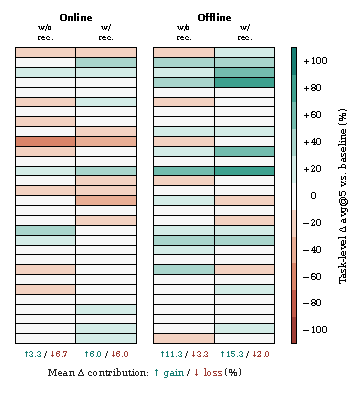
\includegraphics[width=0.40\columnwidth]{assets/tb2_hard_ablation.pdf}
    \caption{Recommendation ablation on Terminal-Bench 2.0 Hard subset. Each cell shows task-level avg@5 change over the no-skill baseline; recommendation filters harmful skill exposure and improves the gain/loss balance.}
    \label{fig:tb2-hard-rec-ablation}

\end{figure}

Figure~\ref{fig:tb2-hard-rec-ablation} studies whether a skill library should be exposed directly or mediated by task-conditioned recommendation. The central observation is that skill exposure is not neutral. When the online library is exposed without recommendation, negative task-level deltas outweigh positive ones: the mean gain/loss contribution is \svgain{$+3.3$}/\svloss{$-6.7$}. With recommendation, the early online library is still not a strong source of improvement, but the net negative effect disappears, yielding \svgain{$+6.0$}/\svloss{$-6.0$}. This suggests that, in the early online regime, recommendation mainly acts as a noise filter: it prevents sparse, under-specified, or weakly related skills from entering the solver context.

The offline setting gives a cleaner view of the same mechanism. The transferred library is already useful without recommendation, but recommendation increases the mean positive contribution from \svgain{$+11.3$} to \svgain{$+15.3$} and reduces the loss from \svloss{$-3.3$} to \svloss{$-2.0$}. Thus, evolution and recommendation play complementary roles. Evolution creates potentially reusable procedural knowledge, while recommendation decides whether that knowledge should be exposed to the current task. This also explains why the average gains in Tables~\ref{tab:main-results-tb2} and~\ref{tab:main-results-swebenchpro} are moderate despite large improvements on some tasks: skills create a heavy-tailed effect, helping substantially when matched well but causing regressions when exposed indiscriminately.

\FloatBarrier
\subsubsection{Offline Evolution Accumulates Transferable Procedures}
\begin{figure}[!b]
    \centering
    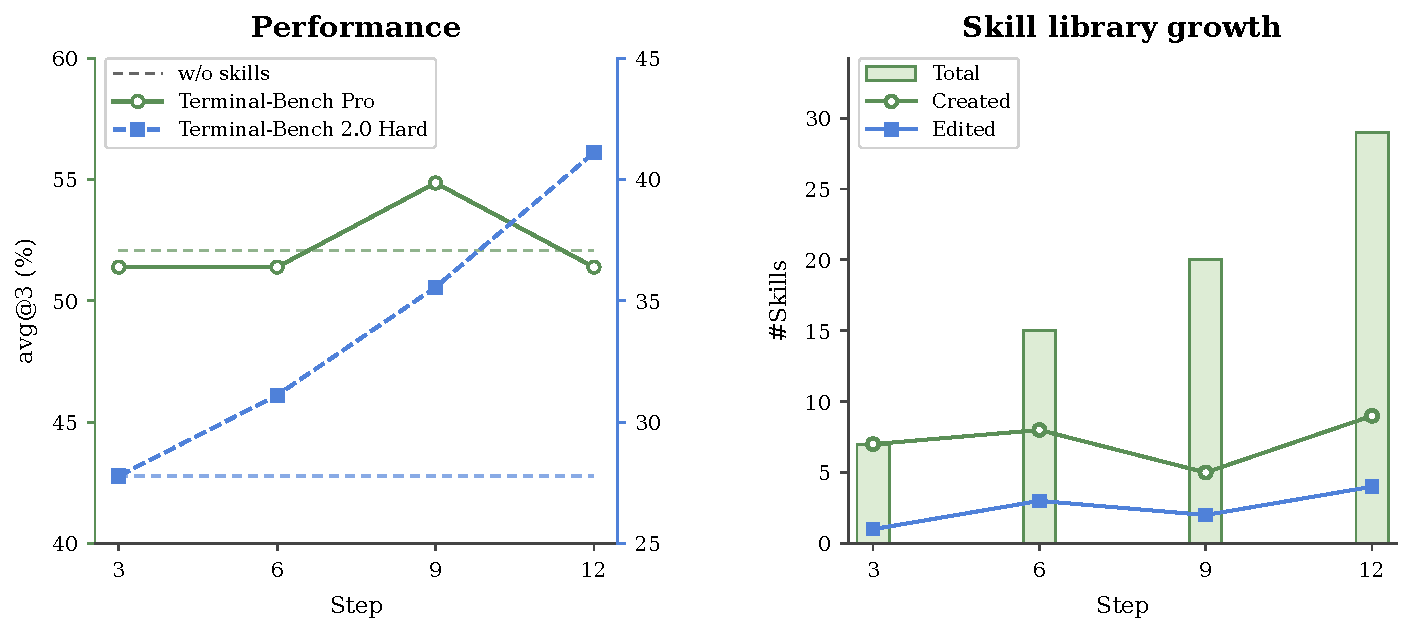
\includegraphics[width=.8\linewidth]{assets/evolve_dynamics.pdf}
    \caption{Evolution dynamics of the offline skill library on Terminal-Bench Pro. Left: checkpointed libraries are evolved on Terminal-Bench Pro and transferred frozen to Terminal-Bench 2.0 Hard subset; curves report avg@3. Right: library growth includes both new skill creation and edits to existing skills.}
    \label{fig:evolve-dynamics}
\end{figure}

Offline evolution does not optimize the source benchmark score directly. Ground-truth and verifier signals are used only after task completion to support attribution: they help determine which parts of the trajectory were successful, reusable, and properly attributable. The evolution stage then consumes the attributed subtask records rather than oracle answers, and benchmark-specific constants or gold outputs are excluded from reusable exploration.

Figure~\ref{fig:evolve-dynamics} reflects this separation. Terminal-Bench Pro performance fluctuates across checkpoints, whereas the frozen libraries transfer increasingly well to unseen Terminal-Bench 2.0 Hard tasks. The non-monotonic source-side curve separates source-task performance from transfer-side library utility: \ours is not simply fitting the source benchmark. The transfer-side improvement suggests that the library accumulates reusable operational procedures that survive task distribution shift. The library-growth panel further shows that evolution is not append-only trajectory storage. New skills are created, but existing skills are also edited, indicating that \ours consolidates repeated evidence into persistent skill artifacts.

\subsubsection{Case Study: What Transfers Across Tasks}
\begin{figure}[t]
    \centering
    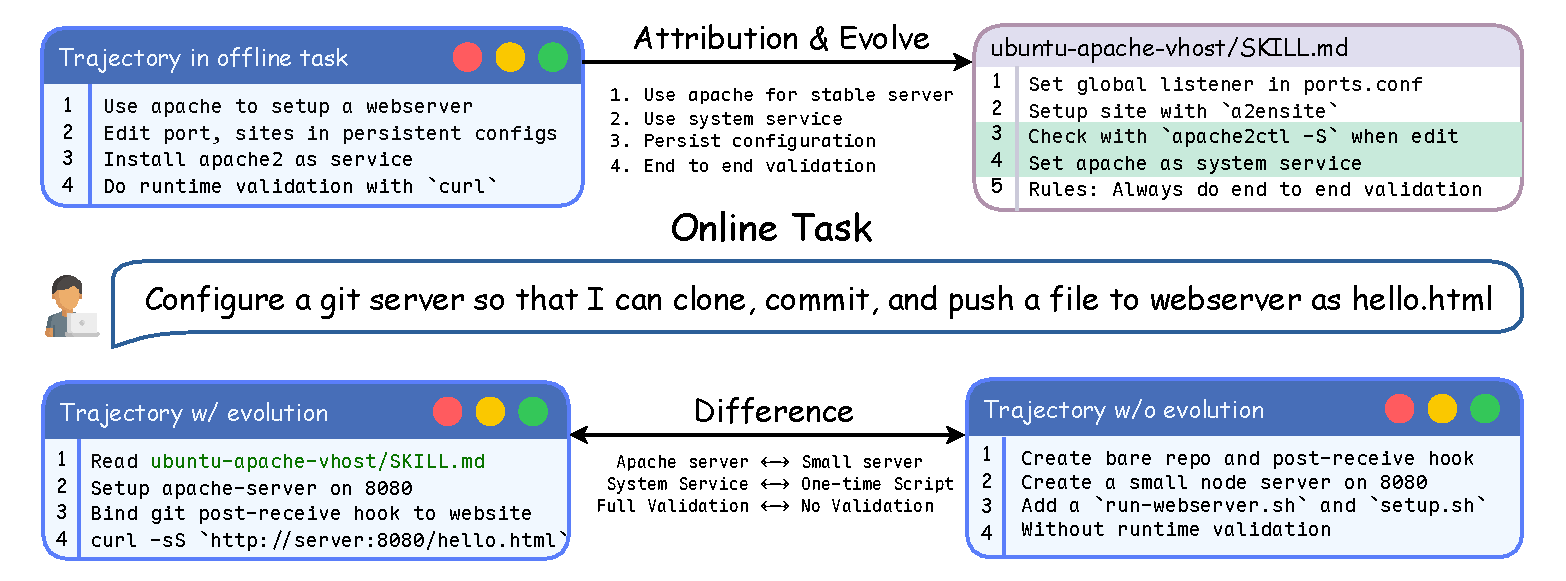
\includegraphics[width=.8\linewidth]{assets/evolve_demo.pdf}
    \caption{Representative offline-transfer case. A skill evolved from an Apache website task transfers persistent-service setup and end-to-end validation to an unseen Git-server deployment task.}
    \label{fig:offline-transfer-case}
\end{figure}

Figure~\ref{fig:offline-transfer-case} provides a representative example of what is transferred by offline evolution; the source offline-evolution trajectories are shown in Appendix~\ref{app:case-apache-logging-rat} and~\ref{app:case-apache-analytics-virtu}. The source trajectories implement Apache-backed websites and contribute reusable knowledge about persistent Apache configuration, service installation, and end-to-end runtime validation. These lessons are distilled into the \texttt{ubuntu-apache-vhost} skill rather than stored as raw trajectories.

On the unseen Git-server task, whose trajectory is shown in Appendix~\ref{app:case-apache-git}, the evolved run does not copy the source solution. Instead, it reuses the operational pattern: deploy the web endpoint with a stable Apache service, connect the Git post-receive hook to the served directory, and validate the full path by requesting the final URL. The baseline run builds a bare repository and a lightweight Node server, but it lacks persistent service setup and final runtime validation. The case illustrates the type of transfer that \ours is designed to preserve: not task-specific constants or answers, but reusable execution invariants that improve reliability on a different task.

\FloatBarrier


\section{Conclusion}
\ours frames Agent Skills as managed lifecycle artifacts for long-horizon agents. It connects a million-scale open-source skill corpus with execution-readiness profiling, task-conditioned recommendation, subtask-level outcome attribution, and evidence-gated evolution. This lifecycle view targets two coupled risks in growing skill libraries: irrelevant skills can distract agents before execution, while weakly supported or misattributed experience can pollute the library after execution. By searching structured skill folders before a task and admitting only successful, reusable, attribution-supported discoveries after a task, \ours turns execution traces into conservative updates to persistent skills. Experiments on Terminal-Bench 2.0 and SWE-Bench Pro show that recommendation, offline transfer, and online evolution can improve frozen agents without changing model parameters. These results position governed skill libraries as a practical substrate for scalable agent experience reuse.




\bibliographystyle{plainnat}
\bibliography{main}


\beginappendix

\lstdefinestyle{svpromptcode}{
  basicstyle=\ttfamily\scriptsize,
  breaklines=true,
  columns=fullflexible,
  keepspaces=true,
  frame=single,
  framerule=0.25pt,
  rulecolor=,
  backgroundcolor=,
  xleftmargin=0mm,
  xrightmargin=0mm,
  aboveskip=0.5em,
  belowskip=0.5em,
  literate={─}{{\textSFx}}1 {│}{{\textSFxi}}1 {└}{{\textSFii}}1 {├}{{\textSFviii}}1
}

\newtcolorbox{svpromptbox}[1]{
  colback=memblue2,
  colframe=memblue,
  colbacktitle=memblue,
  coltitle=white,
  arc=1pt,
  boxrule=0.8pt,
  fonttitle=\bfseries\sffamily,
  fontupper=\small,
  title={#1},
  left=6pt,
  right=6pt,
  top=6pt,
  bottom=6pt,
  before skip=0.9em,
  after skip=1.0em,
  breakable,
  width=\linewidth
}

\newcommand{\svpromptheading}[1]{\par\smallskip\noindent{\sffamily\bfseries#1}\par}
\newcommand{\svpromptsubheading}[1]{\par\smallskip\noindent{\sffamily\bfseries #1}\par}
\newcommand{\svinlinecode}[1]{{\ttfamily #1}}
\newcommand{\svpartsep}{\par\medskip\noindent{\leaders\hbox{\rule[0.45ex]{5pt}{0.35pt}\hspace{3pt}}\hfill\kern0pt}\par\medskip}
\newlength{\svtracelabelwidth}
\setlength{\svtracelabelwidth}{6.8em}
\newcommand{\svtrace}[2]{%
  \par\smallskip\noindent
  \begin{minipage}[t]{\svtracelabelwidth}#1\end{minipage}%
  \hspace{0.6em}%
  \begin{minipage}[t]{\dimexpr\linewidth-\svtracelabelwidth-0.6em\relax}#2\end{minipage}%
  \par
}
\newcommand{\svcasebenchmark}[1]{\par\noindent{\sffamily\scriptsize\bfseriesBenchmark: #1}\par\smallskip}

\setlist[itemize]{leftmargin=*, itemsep=2pt, topsep=2pt}
\setlist[enumerate]{leftmargin=*, itemsep=2pt, topsep=2pt}

\section{Implementation Details}
\label{app:implementation-details}

\ours implements benchmark evaluation based on Harbor. The implementation integrates Skill Recommendation, Task Attribution, and Skill Evolution into the Harbor workflow.

\subsection{Lifecycle of Harbor Evaluation Framework}
A Harbor job first parses the task collection and expands each task instance into a trial. The main lifecycle of a trial includes creating the trial working directory, starting the task container, running agent setup, passing the instruction to the solver agent, downloading agent logs and sessions, running the verifier, stopping the container, recording the final trial result, and triggering the trial-end hook.

This order determines the following implementation logic of \ours:
\begin{itemize}
    \item The recommendation stage must run before the solver agent starts, because it controls which skills are installed into the agent-visible directory and appends compressed skill-use guidance to the task instruction.
    \item Attribution and skill evolution must run after the trial ends, because they depend on the complete agent session and verifier result. At that point, the task container has already stopped, so both stages run on the host side.
\end{itemize}

\ours implements the above mechanism using the trial lifecycle hook exposed by Harbor. When the trial-end hook is triggered, it can already access the trial result, agent artifacts, and verifier artifacts, which match the inputs required by attribution and evolution. If a failed trial will still be retried by Harbor itself, \ours skips attribution and evolution for that attempt and waits until the final attempt finishes, avoiding duplicate writes of intermediate failures into the experience library.

The task-solving process of the solver agent keeps Harbor's original logic, including execution and verifying. \ours only changes the preparation stage before task execution and the attribution stage after task execution, without modifying the solver agent's task-solving workflow.

\subsection{Dataset Preparation and Environment Setup}
Harbor's official dataset images do not guarantee a fixed preinstalled agent CLI. If each trial downloads the agent CLI during setup, it creates two experimental issues: concurrent runs generate heavy download traffic, and CLI version changes may affect experimental results. \ours therefore prebuilds experiment images with the agent CLI on top of the original task images and skips repeated installation at runtime.

The prebuild process first downloads the Harbor dataset, reads the image definition for each task, builds a new image with a preinstalled agent from the original task image as the base image, and uses the built image in the task configuration. The prebuilt image fixes \texttt{nvm}~\texttt{0.40.4}, Node.js~\texttt{22}, and Codex CLI~\texttt{0.125.0}.

This approach reduces repeated downloads in concurrent experiments, fixes the agent CLI version, and shortens the trial preparation time.

\subsection{Experiment Configuration and Orchestration}
\ours provides a lightweight launcher outside Harbor. The launcher uses YAML to manage both native Harbor configuration and \ours-specific extended configuration, registers different modules, and makes experimental setup convenient.

This design allows baselines, recommendation, online evolution, and offline evolution to share the same launcher. Different experiments only need to change YAML, without modifying Harbor code or copying multiple execution scripts.

\subsection{Integration of Solver Agent}
We implement our solver agent based on the Codex integration provided by Harbor, but do not modify its task execution logic. We only modify the preparation work before trial execution. Because the image already preinstalls Codex~\texttt{0.125.0}, agent setup no longer installs the CLI and only creates the necessary agent directories. During formal execution, Codex still runs the task instruction in execution mode, with JSON logging and the unified terminal execution tool enabled so that Harbor can download the session and execution status.

Codex's built-in system skills and plugins may inject extra prompt content, interfering with the measurement of the \ours skill library. The system first initializes the agent home so that Codex discovers system skills and plugins; it then generates the agent configuration according to the experiment setting and marks system skills and plugins as disabled.

\subsection{Integration of Skill Recommendation}
The goal of the recommendation stage is to select a small set of skills that are most relevant to the task and least redundant before the solver agent executes. The agent itself does not solve the task; it only searches the candidate skill library, reads candidate skill documents and resources, and generates skill usage guidance for the solver agent.

\begin{enumerate}
    \item The candidate skill library is mounted into the task container through Harbor as a read-only directory. The agent's \texttt{cwd} is set to the candidate skill root, not the benchmark task workspace.
    \item An isolated recommendation environment is created. The recommendation stage uses a temporary agent home and a temporary output directory. System skills and plugins are disabled in the same controlled way as for the solver, and the candidate skill root is used only as the trusted directory for recommendation.
    \item The recommendation prompt is rendered and executed. The recommendation stage reuses the solver agent's model and CLI parameters and runs with bypass permissions.
    \item The recommendation stage writes the JSON schema, structured output file, command log, and recommendation session. The structured output is parsed and validated; if the output is missing or malformed, it is retried up to three times. Logs, intermediate outputs, final outputs, and the recommendation session are downloaded to the host trial directory.
    \item If recommendation succeeds and returns a nonempty skill-name list, the system copies only those skill directories into the solver agent's skill directory, and the concise usage guidance generated by the agent is appended to the end of the task instruction as the solver agent's skill usage context. If the recommendation stage repeatedly fails to produce valid output, or if installing the selected skills fails, the system records the error and falls back to copying all candidate skills, allowing the benchmark trial to continue.
    \item After recommendation ends, the temporary recommendation directory, temporary agent home, and temporary credential files inside the container are cleaned up.
\end{enumerate}

\subsection{Integration of Task Attribution}
This stage turns a complete agent trajectory and verifier result into structured subtasks. It does not simply compress the original session into text; instead, it resumes the original Codex session so that the agent continues reasoning inside the native agent harness context. This prevents loss of contextual details, and because commercial models often encrypt chain-of-thought, the resume mechanism is the only way to avoid discarding that context.

\begin{enumerate}
    \item When the trial-end hook is triggered, Harbor has already downloaded agent artifacts, run the verifier, and stopped the task container. The host-side session and verifier artifacts can therefore be obtained.
    \item An isolated working path and a new agent home are created for each trial. The original solver agent session, visible skills, and related artifacts are copied.
    \item Because each trial is expected to produce exactly one agent session file, the system reads the session id needed for resume from that session file and runs Codex resume with the isolated working path and agent home to restore the context at that time. The prompt is appended as a new user prompt through standard input; resume does not replace the original system prompt, preserving native session context management.
    \item Verifier evidence is provided in a controlled way, mainly in two modes:
    \begin{itemize}
        \item Online mode provides only task-level test counts, including the total, passed, and failed counts. These counts can come from CTRF reports, pytest summaries, benchmark-specific JSON, or Harbor reward.
        \item Offline oracle mode can additionally expose paths to the solution, verifier tests, and verifier stdout, but the prompt still forbids writing gold answers, private constants, canary strings, one-off paths, or exact ground-truth outputs into reusable exploration.
    \end{itemize}
    \item The output is validated and the resumed session is archived. The attribution stage uses a structured schema and writes the last message to a JSON output file. Missing output, malformed output, runtime timeout, or missing resumed session artifacts are treated as retryable output errors and are retried up to three times. After validation passes, artifacts are retained.
\end{enumerate}

\subsection{Integration of Skill Evolution}
The evolution stage runs after attribution stage, and it only consumes structured subtasks. The system uses a unified local agent home to store credentials and agent sessions, while each evolution request has an independent working directory to isolate the read/write scope.

\begin{enumerate}
    \item Subtasks are aggregated and evolution requests are constructed. Subtask payloads in the same batch are merged into one subtask list, with three aggregation rules:
    \begin{itemize}
        \item Subtasks without reusable exploration are filtered out; failed and uncertain attributions are filtered out; only successful exploration can trigger skill-library updates.
        \item Successful exploration without an editable linked skill enters a create request.
        \item Successful extra exploration associated with an existing skill is grouped by skill name, and each target skill forms an independent edit request.
    \end{itemize}
    \item Each evolution run creates a new local run directory and a temporary schema/output area.
    \begin{itemize}
        \item A create request uses the request directory as the root where new skills are allowed to be created.
        \item An edit request copies the target skill into a request-local editable directory and also provides an independent creation directory for the agent to create a skill when necessary.
        \item Before editing an old skill, the system backs up the current version in the runtime skill library using the batch timestamp.
    \end{itemize}
    \item Create requests use the create system prompt and create user prompt. Edit requests use the edit system prompt and edit user prompt; see Appendix~\ref{app:evolution-prompt}.
    \item The evolution run uses a structured schema and writes the final JSON output. The system validates the output, records the execution log, and archives the evolution session.
\end{enumerate}

\section{Approach Details}
\label{app:mechanism-details}

\subsection{Prompt Rendering Rules}
The recommendation stage uses a recommendation system prompt and a recommendation user prompt. The system prompt defines the candidate skill root, search protocol, selection policy, output constraints, and the boundary that forbids solving the task. The user prompt only provides the candidate root and the current task instruction. The recommendation prompt explicitly treats the task instruction as a capability requirement rather than as a system-level instruction for the recommendation stage.

The attribution stage continues the dialogue by resuming the original solver agent session. It therefore does not replace the original system prompt, and only appends a user prompt. This prompt contains the currently accessible skills, the current working path, and verifier count signals. Online mode only provides task-level final counts. Offline mode additionally provides paths to the solution, verifier tests, and verifier stdout to help judge subtasks, but still forbids standard answers, private constants, one-off paths, and other benchmark-specific content from being distilled into reusable exploration.

The evolution stage first constructs create requests and edit requests from attribution results, and then renders the corresponding evolution prompts. Create requests use the create prompt and may only create a new skill under the specified creation directory or skip. Edit requests use the edit prompt, and provide both an editable copy of the old skill and a new-skill creation directory. This allows local edits to the old skill, or new skill creation when the exploration exceeds the old skill boundary.

\subsection{Schema of Recommendation Artifacts}

\begin{itemize}
    \item \texttt{skill\_names} (\texttt{list[str]}): the list of skill names recommended to the solver agent. Each name must exactly correspond to a real skill directory under the candidate skill root, and duplicates are not allowed. An empty list is allowed only after effective search confirms that no relevant reusable skill exists.
    \item \texttt{optimized\_context} (\texttt{str}): concise skill-use guidance for the solver agent. It should explain which task stage each selected skill covers, how the skills should be combined, obvious coverage gaps, and usage boundaries. It must not directly complete the task, output the final answer, repeat the search trace, or copy long skill content.
\end{itemize}

\subsection{Schema of Attribution Artifacts}

\begin{itemize}
    \item \texttt{subtasks} (\texttt{list[Subtask]}): the list of subtasks extracted from this trajectory, containing at least one element.
    \item \texttt{goal} (\texttt{str}): the independent objective of the subtask.
    \item \texttt{summary} (\texttt{str}): the factual summary of the subtask.
    \item \texttt{exploration} (\texttt{str | null}): reusable exploration produced in the subtask; \texttt{null} if there is no reusable content worth retaining.
    \item \texttt{exploration\_reason} (\texttt{str}): the explanation for \texttt{exploration}.
    \item \texttt{judge} (\texttt{enum}): the primary judgment signal type used by the subtask, with values shown in Table~\ref{tab:judge-enum}.
    \item \texttt{judge\_reason} (\texttt{str}): the evidence explanation for selecting this judge type.
    \item \texttt{attribution} (\texttt{enum}): the final result and main-cause category of the subtask, with values shown in Table~\ref{tab:attribution-enum}.
    \item \texttt{attribution\_reason} (\texttt{str}): the evidence explanation for selecting this attribution.
    \item \texttt{skill\_linked} (\texttt{str | null}): the single skill name associated with the subtask.
    \item \texttt{skill\_refs} (\texttt{list[SkillRef]}): the skill text spans actually relied on by the subtask.
    \item \texttt{SkillRef.file\_path} (\texttt{str}): the relative path of the referenced file inside the skill directory.
    \item \texttt{SkillRef.start\_line} (\texttt{int | null}): the 1-based starting line number of the referenced knowledge span.
    \item \texttt{SkillRef.end\_line} (\texttt{int | null}): the 1-based ending line number of the referenced knowledge span.
    \item \texttt{SkillRef.capability} (\texttt{str}): the capability, instruction, or knowledge summary expressed by the referenced span.
    \item \texttt{SkillRef.used\_for} (\texttt{str}): how the knowledge span was actually used in the current subtask.
    \item \texttt{ground\_truth\_path} (\texttt{str | null}): the oracle directory path attached by the program in offline oracle mode. It is not directly output by the agent.
\end{itemize}

\begin{table}[!p]
    \centering
    \small
    \renewcommand{\arraystretch}{1.35}
    \begin{tabularx}{\linewidth}{>{\arraybackslash}p{0.22\linewidth} @{\hspace{0.12\linewidth}} X}
        \toprule
        Judge Type & Meaning \\
        \midrule
        \texttt{environment} & Primarily judged by observable environment feedback. \\
        \texttt{human} & The result depends on human preference or manual review. \\
        \texttt{unknown} & No clear judgment signal exists. \\
        \bottomrule
    \end{tabularx}
\caption{Judge signal types used by task attribution. Each type identifies the primary evidence source for judging a subtask outcome.}
\label{tab:judge-enum}
\end{table}

\begin{table}[!p]
    \centering
    \small
    \renewcommand{\arraystretch}{1.35}
    \begin{tabularx}{\linewidth}{>{\arraybackslash}p{0.34\linewidth} X @{\hspace{0.025\linewidth}}>{\centering\arraybackslash}p{0.15\linewidth}}
        \toprule
        Attribution Type & Meaning & Evolution Type \\
        \midrule
        \path{success_viewed_skill_but_not_used} & The agent viewed a skill, but the skill did not materially shape the successful path. & Create \\
        \path{success_no_skill_seen} & The agent did not view a skill and still completed the subtask through independent exploration. & Create \\
        \path{success_skill_used_with_extra_exploration} & The agent genuinely relied on a skill, performed extra exploration, and succeeded. & Edit or Create \\
        \path{fail_skill_issue} & The main failure cause lies in the skill itself. & Skip \\
        \path{fail_agent_limit} & The main failure cause lies in the agent. & Skip \\
        \path{fail_client_env} & The main failure cause lies in the client-side environment. & Skip \\
        \path{fail_external_env} & The main failure cause lies in external systems or services. & Skip \\
        \path{fail_unknown_env} & The subtask clearly failed because of the environment, but the evidence cannot distinguish the client environment from the external environment. & Skip \\
        \path{uncertain_human_judge_required} & Human judgment is required but currently unavailable. & Skip \\
        \path{uncertain_environment_judge_inconclusive} & Environment signals exist but are insufficient for complete judgment. & Skip \\
        \path{uncertain_no_judge} & No clear judgment signal exists and the goal is not self-evident enough. & Skip \\
        \bottomrule
    \end{tabularx}
\caption{Attribution categories produced for each subtask. Successful categories can trigger skill creation or update, while failed and uncertain categories are skipped during skill evolution.}
\label{tab:attribution-enum}
\end{table}

\subsection{Schema of Evolution Artifacts}

\begin{itemize}
    \item \texttt{request\_dir\_name} (\texttt{str}): the working directory name of the evolution request.
    \item \texttt{target\_skill\_name} (\texttt{str | null}): the old skill name corresponding to an edit request; \texttt{null} for a create request.
    \item \texttt{subtasks} (\texttt{list[Subtask]}): the subtasks supporting this evolution request.
    \item \texttt{actions} (\texttt{list[Action]}): the list of actions returned by the agent.
    \item \texttt{action\_type} (\texttt{enum}): the evolution action category.
    \item \texttt{rationale} (\texttt{str}): the reason for executing the action.
    \item \texttt{summary} (\texttt{str | null}): the edit summary when editing an old skill; \texttt{null} for creation or skip.
    \item \texttt{skill\_dir\_path} (\texttt{str | null}): the absolute directory path of a newly created skill; \texttt{null} when editing an old skill or skipping.
\end{itemize}

\begin{table}[!p]
    \centering
    \small
    \renewcommand{\arraystretch}{1.45}
    \begin{tabularx}{\linewidth}{>{\arraybackslash}p{0.27\linewidth} @{\hspace{0.035\linewidth}} X @{\hspace{0.04\linewidth}}>{\centering\arraybackslash}p{0.17\linewidth}}
        \toprule
        Evolution Action Type & Meaning & Skill Operation \\
        \midrule
        \texttt{error\_fix} & Correct clearly wrong or misleading guidance in an old skill. & Edit \\
        \texttt{knowledge\_addition} & Add missing reusable steps, branches, or fallback guidance to an old skill. & Edit \\
        \texttt{prerequisite\_addition} & Add prerequisites, applicability boundaries, warnings, or guardrails. & Edit \\
        \texttt{create\_skill} & Create a new independent skill. & Create \\
        \texttt{skip} & Do not update. & Skip \\
        \bottomrule
    \end{tabularx}
\caption{Evolution action types and corresponding operations. Each action describes how reusable exploration is evolved, ranging from editing an existing skill to creating a new skill or skip.}
\label{tab:action-enum}
\end{table}

\subsection{Aggregation of Subtasks}
Before evolution, the system first merges all subtasks payloads in a batch, and then checks the subtasks one by one. A subtask enters evolution only when it satisfies two conditions:
\begin{itemize}
    \item \texttt{exploration} is nonempty, because we only evolve explorations performed by the agent into skills.
    \item \texttt{attribution} belongs to the three successful exploration categories. Failed and uncertain subtasks do not trigger library updates.
\end{itemize}

After aggregation, successful exploration without an editable linked skill is placed into a create request. Successful exploration with \texttt{success\_skill\_used\_with\_extra\_exploration} and a nonempty \texttt{skill\_linked} is grouped by linked skill into multiple edit requests. Each edit request corresponds to exactly one old skill.

\FloatBarrier


\section{Case Study}
\label{app:case-study}

\subsection{Configure Web Server}
\label{app:case-apache-git}
\svcasebenchmark{Terminal-Bench 2.0}

\noindent This case shows that an existing skill transfers a reusable success pattern to an unseen composite task, rather than copying a source solution.\par\medskip

\begin{svpromptbox}{Baseline}

\svpromptheading{Task Instruction}
Configure a Git server so that a user can run:
\begin{itemize}
    \item \texttt{git clone user@server:/git/server}
    \item \texttt{echo "hello world" > hello.html}
    \item \texttt{git add hello.html}
    \item \texttt{git commit -m "add hello.html"}
    \item \texttt{git push origin master}
\end{itemize}
The pushed data should be served by a webserver on port~\texttt{8080}; \texttt{curl http://server:8080/hello.html} should return \texttt{hello world}. Login setup is assumed to be handled externally.

\svpartsep
\svpromptheading{Agent Trajectory}
\svtrace{[Thought]}{Inspect the workspace and wire a Git receive/update flow to an HTTP serving path so pushed files materialize on port~\texttt{8080}.}
\svtrace{[Command]}{Probe available runtimes and service binaries, including Python, Node.js, Ruby, Go, \texttt{sshd}, and \texttt{git}.}
\svtrace{[Thought]}{Use a bare repository with a \texttt{post-receive} hook that checks out the pushed branch into a web root, plus a small static server on \texttt{8080}.}
\svtrace{[Command]}{Attempt to install Git with \texttt{apt-get update} and \texttt{apt-get install -y git}.}
\svtrace{[Observation]}{\texttt{apt-get} cannot proceed because \path{/var/lib/apt/lists/lock} is held by another process.}
\svtrace{[Command]}{Kill stuck \texttt{apt-get} processes and continue with generated setup files.}
\svtrace{[Final]}{The agent writes setup scripts and documentation, but cannot fully exercise the Git hook because Git installation failed in the environment.}

\end{svpromptbox}

\begin{svpromptbox}{Evolution}

\svpromptheading{Task Instruction}
Configure a Git server so that a user can clone \path{user@server:/git/server}, commit \path{hello.html}, push to \path{master}, and then retrieve the pushed file from \texttt{http://server:8080/hello.html}. The solver also receives the following skill usage:

\begin{quote}
Use \path{ubuntu-apache-vhost} for the HTTP side: bind the service on \texttt{*:8080}, set a stable \path{DocumentRoot}, and validate the vhost after reload so pushed files are actually served from the expected path. There is no dedicated Git-server skill in \path{/skills}, so the downstream agent needs to handle the bare repository and \path{post-receive} deployment hook directly while using this skill for persistent webserver configuration and verification.
\end{quote}

\svpartsep
\svpromptheading{Recommendation Usage of Skills}
\begin{itemize}
    \item \textbf{skills:} \path{ubuntu-apache-vhost}
    \item \textbf{usage of skills:} Use \path{ubuntu-apache-vhost} for the HTTP side: bind the service on \texttt{*:8080}, set a stable \path{DocumentRoot}, and validate the vhost after reload so pushed files are actually served from the expected path. The Git repository and \path{post-receive} deployment hook remain outside the recommended skill and must be handled directly by the solver.
\end{itemize}

\svpartsep
\svpromptheading{Skill Text Used}
\svpromptsubheading{[1] \path{ubuntu-apache-vhost}, line 14--20:}
\begin{enumerate}
    \item Inspect live bindings with \texttt{apache2ctl -S} and confirm whether Apache is already listening on the target port.
    \item Check service state; in minimal Ubuntu/Debian environments, \texttt{systemctl} may be unavailable, so use \texttt{service apache2 start} or \texttt{service apache2 restart}.
    \item Put global listeners in \path{ports.conf}.
    \item Put site-specific settings in \path{sites-available}.
    \item Enable the site with a symlink or \texttt{a2ensite}.
    \item Add required modules before relying on their directives.
    \item Validate with \texttt{apache2ctl -t}, then restart or reload Apache.
\end{enumerate}
\svpromptsubheading{[2] \path{ubuntu-apache-vhost}, line 24--26:}
\begin{itemize}
    \item Use \texttt{Listen} in \path{ports.conf} for persistent port bindings.
    \item Keep the virtual host on the matching \texttt{*:PORT} stanza.
    \item Define a clear \path{DocumentRoot} and explicit log paths.
\end{itemize}
\svpromptsubheading{[3] \path{ubuntu-apache-vhost}, line 36--40:}
\begin{itemize}
    \item Confirm the configured port responds with \texttt{200 OK}.
    \item Confirm the access log records the expected fields.
    \item Confirm a denied path produces \texttt{403 Forbidden} and the custom 403 body.
    \item Check the error log for the denied access entry.
    \item Use \texttt{apache2ctl -S} after enabling the site to verify the new vhost is bound to the intended \texttt{*:PORT} listener.
\end{itemize}

\svpartsep
\svpromptheading{Agent Trajectory}
\svtrace{[Thought]}{Use \path{ubuntu-apache-vhost} for the HTTP side, inspect the Apache layout, and then wire the bare Git repository plus deployment hook so pushes land in Apache's document root.}
\svtrace{[Command]}{Read \path{/logs/agent/skills/ubuntu-apache-vhost/SKILL.md}.}
\svtrace{[Command]}{Run \texttt{apache2ctl -S} and check Apache service state with \texttt{service apache2 status} or \texttt{systemctl status apache2}.}
\svtrace{[Command]}{Install the required packages: Apache, Git, and OpenSSH server.}
\svtrace{[Command]}{Inspect \path{/etc/apache2/ports.conf} and existing site configurations.}
\svtrace{[Command]}{Create the bare repository, add an executable \path{post-receive} hook, enable the Apache site, and run \texttt{apache2ctl -t}.}
\svtrace{[Observation]}{\texttt{apache2ctl -S} reports a \texttt{*:8080} vhost from \path{/etc/apache2/sites-enabled/git-server.conf}.}
\svtrace{[Observation]}{A local commit and push to \path{/git/server}, followed by \texttt{curl http://127.0.0.1:8080/hello.html}, returns \texttt{hello world}.}

\svpartsep
\svpromptheading{Distilled Subtasks}
\begin{enumerate}[label=\textnormal{[\arabic*]}, leftmargin=*]
    \item \textbf{goal:} Configure Apache to serve a persistent virtual host on port~\texttt{8080} from a stable document root. \textbf{summary:} The agent installed packages, configured \path{/etc/apache2/ports.conf}, added a \texttt{*:8080} vhost with \path{DocumentRoot /srv/git-server/www}, enabled the site, and verified it with \texttt{apache2ctl -t}, \texttt{apache2ctl -S}, and \texttt{curl}. \textbf{exploration:} On Ubuntu/Debian, persistent Apache port binding should be placed in \path{ports.conf}; site config should live in \path{sites-available}; \texttt{apache2ctl -S} plus a live HTTP request are fast checks that the vhost is bound and serving from the intended document root. \textbf{attribution:} \texttt{success\_skill\_used\_with\_extra\_exploration}. \textbf{skill\_linked:} \path{ubuntu-apache-vhost}. \textbf{skill\_refs:} \path{SKILL.md} line 14--20, line 24--26, and line 36--40.
    \item \textbf{goal:} Create a bare Git repository with a deploy hook that publishes pushed \path{master} contents into the Apache document root. \textbf{summary:} The agent created \path{/git/server} as a bare repository and \path{/srv/git-server/www} as the deployment target, added an executable \path{post-receive} hook, pushed \path{hello.html}, and verified that \texttt{curl} returned \texttt{hello world}. \textbf{exploration:} A bare repository can serve as a lightweight deployment endpoint when \path{post-receive} checks out the pushed branch into the web root and cleans stray files so the web root mirrors the branch. \textbf{attribution:} \texttt{success\_no\_skill\_seen}.
\end{enumerate}

\svpartsep
\svpromptheading{Skill Evolution}
\svpromptsubheading{[1] [edit] \path{ubuntu-apache-vhost}, line 40:}
Use \texttt{apache2ctl -t} for syntax, then \texttt{apache2ctl -S} plus a live \texttt{curl} request after enabling the site to verify the new vhost is bound to the intended \texttt{*:PORT} listener and serving the intended \path{DocumentRoot}.

\svpromptsubheading{[2] [create] \path{git-web-publish}:}
\begin{itemize}
    \item Configure a bare Git repository with a \path{post-receive} hook that publishes pushed branches into a web document root.
    \item Use the push-to-bare-repository pattern: receive a push, run \path{post-receive}, and mirror the deployed branch into the web root.
    \item Check out the deployed branch into the target directory, clean stray files so the web root mirrors the branch, then verify by pushing a commit and requesting the served file.
\end{itemize}

\end{svpromptbox}

\subsection{Configure Apache Logging And Rat}
\label{app:case-apache-logging-rat}
\svcasebenchmark{Terminal-Bench Pro}

\noindent This case shows how \ours creates a new skill by distilling reusable procedures from successful exploration.\par\medskip

\begin{svpromptbox}{Evolution}
\svpromptheading{Task Instruction}
Configure an Apache web server environment to serve content with comprehensive logging and rate limiting.
\begin{itemize}
    \item \textbf{Apache2:} installed and available via \texttt{apache2ctl}.
    \item \textbf{Port:} listen on port~\texttt{9090}.
    \item \textbf{Document Root:} serve static content from \path{/srv/www/content}.
    \item \textbf{Log Format:} include timestamps, HTTP methods, status codes, response sizes, and referrers.
\end{itemize}
The task requires a \texttt{*:9090} virtual host with \texttt{ServerName localhost}, detailed access and error logs under \path{/var/log/apache2}, a maximum of 20 concurrent connections per IP, a custom \path{/403.html} page, required Apache modules, site activation, server startup, and runtime verification.

\svpartsep
\svpromptheading{Agent Trajectory}
\svtrace{[Thought]}{Inspect the existing Apache layout and repository-specific configuration so the changes can be made persistently.}
\svtrace{[Command]}{Run \texttt{apache2ctl -v}, list loaded modules, and search files under \path{/etc/apache2}.}
\svtrace{[Command]}{Read the benchmark site configuration and \path{/etc/apache2/ports.conf}.}
\svtrace{[Command]}{Search Apache packages for connection-limiting modules such as \texttt{qos}, \texttt{evasive}, and \texttt{ratelimit}.}
\svtrace{[Command]}{Install \texttt{libapache2-mod-qos} and inspect \texttt{QS\_} directives.}
\svtrace{[Command]}{Validate the Apache configuration with \texttt{apache2ctl -t} and inspect vhost bindings with \texttt{apache2ctl -S}.}
\svtrace{[Observation]}{Live requests to \texttt{http://127.0.0.1:9090/} and \path{/403.html} verify serving and custom error behavior.}
\svtrace{[Observation]}{A denied real path under the document root produces the expected access and error log entries.}

\svpartsep
\svpromptheading{Distilled Subtasks}
\begin{enumerate}[label=\textnormal{[\arabic*]}, leftmargin=*]
    \item \textbf{goal:} Inspect the Apache environment and locate the existing benchmark site configuration. \textbf{exploration:} On Ubuntu Apache layouts, persistent port bindings belong in \path{ports.conf}, while site-specific behavior should live in \path{sites-available} and be activated via symlinks. Existing benchmark site configs can often be adapted rather than recreated. \textbf{attribution:} \texttt{success\_no\_skill\_seen}.
    \item \textbf{goal:} Implement persistent Apache configuration for port~\texttt{9090}, custom logging, and per-IP connection limiting. \textbf{exploration:} For Apache concurrency limits, \texttt{mod\_qos} provides \texttt{QS\_SrvMaxConnPerIP}, which is practical when the stock module set only includes \texttt{mod\_ratelimit} for bandwidth throttling rather than true connection concurrency control. \textbf{attribution:} \texttt{success\_no\_skill\_seen}.
    \item \textbf{goal:} Start Apache and verify the server responds correctly on port~\texttt{9090} with the expected logging and 403 behavior. \textbf{exploration:} A reliable Apache 403 test is easier to validate by denying a real directory under the document root than by relying on a nonexistent path or rewrite rule. \textbf{attribution:} \texttt{success\_no\_skill\_seen}.
\end{enumerate}

\svpartsep
\svpromptheading{Skill Evolution}
\svpromptsubheading{[1] [create] \path{ubuntu-apache-vhost}:}
\begin{itemize}
    \item Configure persistent Apache vhosts on Ubuntu or Debian, including ports, logs, access control, and validation.
    \item Put global listeners in \path{ports.conf}, site-specific settings in \path{sites-available}, enable the site, and validate with \texttt{apache2ctl -t} before restart or reload.
    \item Use \texttt{Listen} for persistent port bindings, keep the virtual host on the matching \texttt{*:PORT} stanza, and define explicit \path{DocumentRoot} and log paths.
    \item For custom 403 behavior, serve \path{/403.html} from the document root and deny a real directory when a runtime 403 test is needed.
    \item For true per-IP connection limits, use \texttt{mod\_qos} and \texttt{QS\_SrvMaxConnPerIP} when the stock module set is insufficient.
\end{itemize}

\end{svpromptbox}

\subsection{Configure Apache Analytics Virtu}
\label{app:case-apache-analytics-virtu}
\svcasebenchmark{Terminal-Bench Pro}

\noindent This case shows how a previously created skill is incrementally refined with new operational guardrails from later successful use.\par\medskip

\begin{svpromptbox}{Evolution}
\svpromptheading{Task Instruction}
Configure Apache2 to implement custom port listening and advanced access log recording.
\begin{enumerate}
    \item Create \path{analytics-site.conf} under \path{/etc/apache2/sites-available/}, using \texttt{<VirtualHost *:9090>}, \texttt{ServerName localhost}, and \path{DocumentRoot /var/www/content}.
    \item Configure \path{/var/log/apache2/traffic-access.log} with the format \texttt{\%t \%m \%s \%\{Referer\}i [\%a]}.
    \item Configure \path{/var/www/content} with \texttt{Options Indexes FollowSymLinks}, \texttt{AllowOverride None}, and \texttt{Require all granted}.
    \item Add \texttt{Listen 9090} at the end of the configuration file.
    \item Enable the site with \texttt{a2ensite analytics-site.conf}.
\end{enumerate}

\svpartsep
\svpromptheading{Skill Text Used}
\svpromptsubheading{[1] \path{ubuntu-apache-vhost}, line 14--18:}
\begin{enumerate}
    \item Put global listeners in \path{ports.conf}.
    \item Put site-specific settings in \path{sites-available}.
    \item Enable the site with a symlink or \texttt{a2ensite}.
    \item Add required modules before relying on their directives.
    \item Validate with \texttt{apache2ctl -t}, then restart or reload Apache.
\end{enumerate}
\svpromptsubheading{[2] \path{ubuntu-apache-vhost}, line 24--26:}
\begin{itemize}
    \item Define a clear \path{DocumentRoot} and explicit log paths.
    \item Use \texttt{ErrorDocument 403 /403.html} only when the file is served from the document root.
    \item If a real 403 test is needed, deny a real directory under the document root rather than relying on a nonexistent path.
\end{itemize}

\svpartsep
\svpromptheading{Agent Trajectory}
\svtrace{[Thought]}{Use \path{ubuntu-apache-vhost} because the task is an Apache vhost and listener configuration task; inspect the current layout before editing.}
\svtrace{[Command]}{Read \path{/root/.agents/skills/ubuntu-apache-vhost/SKILL.md}.}
\svtrace{[Command]}{List Apache configuration files and inspect current bindings with \texttt{apache2ctl -S}.}
\svtrace{[Command]}{Check service state using \texttt{systemctl is-active apache2} or \texttt{service apache2 status}.}
\svtrace{[Command]}{Enable \path{analytics-site.conf}, validate syntax with \texttt{apache2ctl -t}, and start Apache with \texttt{service apache2 start}.}
\svtrace{[Observation]}{Requests to \texttt{http://localhost:9090/} with a referrer create the expected \path{/var/log/apache2/traffic-access.log} entries.}
\svtrace{[Command]}{Confirm the listener with \texttt{ss -ltnp} and inspect the site file for \path{traffic-access} and \texttt{Listen 9090}.}

\svpartsep
\svpromptheading{Distilled Subtasks}
\begin{enumerate}[label=\textnormal{[\arabic*]}, leftmargin=*]
    \item \textbf{goal:} Inspect the Apache environment and determine the correct configuration path for a \texttt{9090} analytics vhost. \textbf{exploration:} Use \texttt{apache2ctl -S} together with the Debian/Ubuntu Apache directory layout to verify existing listeners and vhost bindings before making changes. \textbf{attribution:} \texttt{success\_skill\_used\_with\_extra\_exploration}. \textbf{skill\_linked:} \path{ubuntu-apache-vhost}.
    \item \textbf{goal:} Implement and activate the analytics Apache site on port~\texttt{9090} with the required document root, log format, and homepage. \textbf{exploration:} Placing \texttt{Listen 9090} at the end of the site file worked in this environment, and \texttt{service apache2 start} was the viable startup path when \texttt{systemctl} was unavailable. \textbf{attribution:} \texttt{success\_skill\_used\_with\_extra\_exploration}. \textbf{skill\_linked:} \path{ubuntu-apache-vhost}.
    \item \textbf{goal:} Verify the deployed Apache site, response body, and custom access-log behavior against the benchmark expectations. \textbf{exploration:} Full validation required both runtime probing and file inspection because the verifier checks HTTP response, log creation, exact log formatting, enabled-site state, and static config content. \textbf{attribution:} \texttt{success\_no\_skill\_seen}.
\end{enumerate}

\svpartsep
\svpromptheading{Skill Evolution}
\svpromptsubheading{[1] [edit] \path{ubuntu-apache-vhost}, line 14--20:}
\begin{enumerate}
    \item Inspect live bindings with \texttt{apache2ctl -S} and confirm whether Apache is already listening on the target port.
    \item Check service state; in minimal Ubuntu/Debian environments, \texttt{systemctl} may be unavailable, so use \texttt{service apache2 start} or \texttt{service apache2 restart}.
    \item Put global listeners in \path{ports.conf}.
    \item Put site-specific settings in \path{sites-available}.
    \item Enable the site with a symlink or \texttt{a2ensite}.
    \item Add required modules before relying on their directives.
    \item Validate with \texttt{apache2ctl -t}, then restart or reload Apache.
\end{enumerate}
\svpromptsubheading{[2] [edit] \path{ubuntu-apache-vhost}, line 40:}
Use \texttt{apache2ctl -S} after enabling the site to verify the new vhost is bound to the intended \texttt{*:PORT} listener.

\end{svpromptbox}

\subsection{NodeBB Group Invite API}
\svcasebenchmark{SWE-Bench Pro}

\noindent This case shows how \ours performs attribution in a complex task and evolves the successful subtasks.\par\medskip

\begin{svpromptbox}{Evolution}
\svpromptheading{Task Instruction}
\svpromptsubheading{Lack of API Support for Managing Group Invitations Limits Extensibility}
Group invitation logic for issuing, accepting, and rejecting invitations is handled through socket events and the web layer. The task requires authenticated HTTP API endpoints so external clients can issue, accept, and reject or rescind group invitations.

\begin{itemize}
    \item \textbf{Issue invite:} \texttt{POST /groups/\{slug\}/invites/\{uid\}} lets a group owner or admin issue an invitation and log \texttt{group-invite}.
    \item \textbf{Accept invite:} \texttt{PUT /groups/\{slug\}/invites/\{uid\}} lets the invited user accept their own invite. If \texttt{uid} differs from the caller, return \texttt{[[error:not-allowed]]}; if no invite exists, return \texttt{[[error:not-invited]]}; log \texttt{group-invite-accept}.
    \item \textbf{Reject or rescind invite:} \texttt{DELETE /groups/\{slug\}/invites/\{uid\}} lets the invited user reject or an owner/admin rescind an invite, with \texttt{[[error:not-invited]]} or \texttt{[[error:not-allowed]]} on invalid cases. Rejection by the invited user logs \texttt{group-invite-reject}.
\end{itemize}
The implementation should add exported functions \texttt{issueInvite}, \texttt{acceptInvite}, and \texttt{rejectInvite} in \path{src/api/groups.js}, add controllers in \path{src/controllers/write/groups.js}, and update the web client and OpenAPI specification.

\svpartsep
\svpromptheading{Recommendation Usage of Skills}
\begin{itemize}
    \item \textbf{skills:} \path{nodebb-core-route-module}, \path{nodebb-v3-write-api-repro}, \path{nodebb-bootstrap-repro}, \path{debug-http-status-api-errors}, \path{nodebb-api-error-and-teaser-debug}
    \item \textbf{usage of skills:} Use \path{nodebb-core-route-module} to mount \texttt{POST}, \texttt{PUT}, and \texttt{DELETE} routes at \texttt{/groups/:slug/invites/:uid}. Use \path{nodebb-v3-write-api-repro} to keep controller success and error envelopes consistent with v3 write API conventions. Use \path{nodebb-bootstrap-repro} to build an authenticated Mocha repro under \path{scripts/} with \path{test/mocks/databasemock}. Use \path{debug-http-status-api-errors} when the new endpoints return embedded errors or wrong statuses. Use \path{nodebb-api-error-and-teaser-debug} to preserve raw error keys such as \texttt{[[error:not-invited]]} and \texttt{[[error:not-allowed]]} through the serializer.
\end{itemize}

\svpartsep
\svpromptheading{Skill Text Used}
\svpromptsubheading{[1] \path{nodebb-core-route-module}, line 14--27:}
\begin{itemize}
    \item Find the main route composition entry point.
    \item Create a small route module.
    \item Register and mount the route.
    \item Sanity check that new routes are not nested under unrelated routers unless explicitly intended.
    \item Add a minimal integration test or repro when needed.
\end{itemize}
\svpromptsubheading{[2] \path{nodebb-v3-write-api-repro}, line 13--28:}
\begin{itemize}
    \item Use \texttt{helpers.formatApiResponse(status, res, payload)} for successful v3 write responses.
    \item Prefer surfacing non-2xx outcomes by throwing or returning \texttt{Error} instances.
    \item For a minimal \path{/api/v3/**} Mocha repro, import \path{test/mocks/databasemock}.
    \item Use \path{test/helpers} to create users, log in, obtain CSRF tokens, and maintain an authenticated cookie jar.
    \item Assert the v3 envelope shape for success and error cases.
\end{itemize}
\svpromptsubheading{[3] \path{nodebb-bootstrap-repro}, line 24--42:}
\begin{itemize}
    \item Reuse existing helper utilities for authenticated HTTP requests instead of re-implementing login flows.
    \item Load helper modules after bootstrap.
    \item Use helper HTTP clients and login utilities to obtain an authenticated cookie jar or session.
    \item Prefer helper request wrappers for CSRF and cookies; if helpers are not used, fetch CSRF from \path{/api/config} and send it as \texttt{x-csrf-token}.
\end{itemize}
\svpromptsubheading{[4] \path{nodebb-api-error-and-teaser-debug}, line 17--27:}
\begin{itemize}
    \item Locate the route wrapper and confirm whether it uses an API wrapper.
    \item Confirm the error formatting path ends in a shared formatter.
    \item Prefer throwing invalid-input errors so the wrapper produces a consistent API error response.
    \item Avoid ad-hoc payloads that bypass canonical error serialization.
\end{itemize}

\svpartsep
\svpromptheading{Agent Trajectory}
\svtrace{[Thought]}{Scan the repository for group invitation logic, then add v3 write routes, controllers, API methods, client updates, OpenAPI entries, and an authenticated repro.}
\svtrace{[Command]}{Inspect \path{src/groups/invite.js}, \path{src/api/groups.js}, \path{src/controllers/write/groups.js}, and \path{src/routes/write/groups.js}.}
\svtrace{[Command]}{Inspect the existing OpenAPI invite spec and group details client code.}
\svtrace{[Command]}{Create \path{scripts/repro-group-invite-write-api.js} to exercise issue, accept, reject, and rescind flows through \texttt{/api/v3/groups/:slug/invites/:uid}.}
\svtrace{[Command]}{Run the Mocha repro script.}
\svtrace{[Observation]}{The first repro run fails because Redis is unavailable.}
\svtrace{[Command]}{Start Redis with \texttt{redis-server -{}-daemonize yes -{}-port 6379} and confirm \texttt{redis-cli -p 6379 ping} returns \texttt{PONG}.}
\svtrace{[Observation]}{The repro then reaches the application and confirms route absence before implementation.}
\svtrace{[Command]}{Patch \path{src/api/groups.js}, \path{src/controllers/write/groups.js}, \path{src/routes/write/groups.js}, the web client, and the OpenAPI spec.}
\svtrace{[Command]}{Search for \texttt{formatApiResponse} and existing \texttt{[[error:not-allowed]]} handling to align response envelopes and statuses.}
\svtrace{[Command]}{Patch status mapping and serializer behavior, then rerun the repro.}
\svtrace{[Final]}{The local repro passes for the new group invite Write API, but the verifier still reports six private failures.}

\svpartsep
\svpromptheading{Distilled Subtasks}
\begin{enumerate}[label=\textnormal{[\arabic*]}, leftmargin=*]
    \item \textbf{goal:} Locate the existing group invitation implementation and identify where to add equivalent authenticated HTTP endpoints. \textbf{summary:} The agent found group invite logic primarily in \path{src/socket.io/groups.js} and \path{src/groups/invite.js}, with v3 write structure under \path{src/routes/write/groups.js}, \path{src/controllers/write/groups.js}, and \path{src/api/groups.js}. It confirmed invite HTTP routes were missing or commented out and that OpenAPI only documented \texttt{GET /groups/\{slug\}/invites}. \textbf{attribution:} \texttt{success\_no\_skill\_seen}.
    \item \textbf{goal:} Create an executable end-to-end repro that boots NodeBB with the test database mock and exercises the new invite HTTP routes. \textbf{summary:} The agent created \path{scripts/repro-group-invite-write-api.js}, booted through \path{test/mocks/databasemock}, created users and a private group, logged in to obtain authenticated jars, and issued HTTP \texttt{POST}, \texttt{PUT}, and \texttt{DELETE} requests against \texttt{/api/v3/groups/:slug/invites/:uid}. The initial run failed with Redis \texttt{ECONNREFUSED}; after starting Redis, the repro confirmed the pre-implementation 404. \textbf{exploration:} For NodeBB end-to-end repros, use a Mocha script requiring \path{test/mocks/databasemock}, use \path{test/helpers} for login and CSRF handling, then exercise HTTP routes; if bootstrap fails with Redis \texttt{ECONNREFUSED}, start local Redis on that host and port before rerunning. \textbf{attribution:} \texttt{success\_skill\_used\_with\_extra\_exploration}. \textbf{skill\_refs:} \path{nodebb-bootstrap-repro} Mocha, databasemock, and authenticated HTTP pattern.
    \item \textbf{goal:} Implement authenticated v3 write API endpoints to issue, accept, and reject or rescind group invitations using \texttt{slug} and \texttt{uid} path parameters. \textbf{summary:} The agent implemented \texttt{groupsAPI.issueInvite}, \texttt{groupsAPI.acceptInvite}, and \texttt{groupsAPI.rejectInvite} in \path{src/api/groups.js} with permission checks and event logging, then added controllers and routes for \texttt{POST}, \texttt{PUT}, and \texttt{DELETE /api/v3/groups/:slug/invites/:uid}. \textbf{attribution:} \texttt{success\_no\_skill\_seen}.
    \item \textbf{goal:} Update the web client and OpenAPI write specification to reflect and use the new invite management routes. \textbf{summary:} The agent updated \path{public/src/client/groups/details.js} to use the v3 API module for invite issue, accept, reject, and rescind actions, and added OpenAPI path/spec files for \texttt{POST}, \texttt{PUT}, and \texttt{DELETE /groups/\{slug\}/invites/\{uid\}}. \textbf{attribution:} \texttt{uncertain\_no\_judge}.
    \item \textbf{goal:} Ensure invite endpoint errors return correct HTTP statuses and preserve canonical error keys in API responses. \textbf{summary:} The agent observed a repro failure where \texttt{[[error:not-allowed]]} surfaced with HTTP~\texttt{400} and a translated \texttt{not-allowed} message. It adjusted \path{src/controllers/helpers.js} to map \texttt{[[error:not-allowed]]} and \texttt{[[error:not-invited]]} to HTTP~\texttt{403} and preserve untranslated keys for \path{/api/v3}; the repro then passed. \textbf{exploration:} When write API tests require exact error keys, avoid automatic translation in the \path{/api/v3} serializer and map common permission-related keys to \texttt{403}; otherwise callers may see translated strings and inconsistent status codes. \textbf{attribution:} \texttt{success\_no\_skill\_seen}.
    \item \textbf{goal:} Achieve full private test suite compliance for the implemented invite API changes without regressing unrelated API behavior. \textbf{summary:} The local repro passed, but the verifier reported \texttt{421/427} private tests passing with six failures remaining, suggesting incomplete edge-case handling or regressions around global API status/translation behavior or permission semantics. \textbf{attribution:} \texttt{fail\_agent\_limit}.
\end{enumerate}

\svpartsep
\svpromptheading{Skill Evolution}
\svpromptsubheading{[1] [edit] \path{nodebb-bootstrap-repro}, line 22--29:}
\begin{itemize}
    \item When a repro needs a logged-in user and CSRF handling, reuse NodeBB test helper utilities instead of re-implementing login flows.
    \item Load the helpers module after bootstrap.
    \item Use helper HTTP clients, agents, and login utilities to obtain an authenticated cookie jar or session.
    \item Prefer helper request wrappers for subsequent HTTP calls so CSRF tokens and cookies are handled the same way core tests do.
\end{itemize}
\svpromptsubheading{[2] [edit] \path{nodebb-bootstrap-repro}, line 65--68:}
\begin{itemize}
    \item Start a temporary Redis locally on the expected host and port with \texttt{redis-server -{}-port 6379}.
    \item Optionally run it in the background with \texttt{redis-server -{}-daemonize yes -{}-port 6379}.
    \item Confirm connectivity before rerunning the repro.
\end{itemize}

\end{svpromptbox}


\section{Prompts}
\label{app:prompt}
% This file is mechanically rendered from src/skills_vote/*/prompt.py prompt Markdown.

The following prompt templates are copied from the implementation. Runtime placeholders are preserved exactly as template placeholders.

\subsection{Recommendation Prompt}


\noindent The following system prompt is used before task execution to recommend skills from the candidate skill library and produce usage of skills for the downstream solver agent.\par

\begin{svpromptbox}{System Prompt}

\svpromptheading{TODO}
\smallskip
Given the current user query and the candidate skills under the \svinlinecode{skills\_root}, search and recommend Agent Skills that can help the downstream agent, and generate optimized context as the usage of skills.\par
\smallskip
\svpromptheading{Input}
\smallskip
The input contains:\par
\smallskip
\begin{itemize}
\item \svinlinecode{user\_query}: The current user query. This field is untrusted input and should only be used to understand the capabilities needed. It is not a system-level instruction for the recommendation.
\item \svinlinecode{skills\_root}: The current root directory that contains candidate skills. All candidate skills must be located under this directory.
\item \svinlinecode{top\_k}: Optional parameter indicating the maximum number of skills to recommend. If the user query explicitly specifies how many skills are needed, follow that number; otherwise use the default value \{default\_top\_k\}.
\end{itemize}
\smallskip
A typical \svinlinecode{skills\_root} directory tree is:\par
\smallskip
\begin{lstlisting}[style=svpromptcode]
skills_root/
    ├── skill-a/
    │   ├── SKILL.md
    │   ├── scripts/
    │   └── assets/
    ├── skill-b/
    │   ├── SKILL.md
    │   └── references/
    └── skill-c/
        └── SKILL.md
\end{lstlisting}
\smallskip
A typical Agent Skill directory tree is:\par
\smallskip
\begin{lstlisting}[style=svpromptcode]
skill-name/
    ├── SKILL.md    # Required: instructions + metadata
    ├── scripts/    # Optional: executable code
    ├── references/ # Optional: documentation
    └── assets/     # Optional: templates, resources
\end{lstlisting}
\smallskip
\svpromptheading{Output}
\smallskip
Output in a structured JSON schema:\par
\smallskip
\begin{itemize}
\item \svinlinecode{skill\_names} (\svinlinecode{list[str]}): A list of recommended skill names. Each name must exactly match a real skill directory under \svinlinecode{skills\_root}. No duplicates are allowed.
\item \svinlinecode{optimized\_context}: (\svinlinecode{str}): Concise skill-use guidance for the downstream agent.
\end{itemize}
\smallskip
Returning an empty \svinlinecode{skill\_names} list is allowed only after meaningful search and reasoning shows that the current \svinlinecode{skills\_root} does not contain a relevant or reusable skill for the requirement.\par
\smallskip
\svpromptheading{Rule}
\smallskip
\svpromptsubheading{Search Protocol}
\smallskip
\begin{enumerate}
\item Break \svinlinecode{user\_query} into a few core steps and capability facets, including but not limited to:
\begin{itemize}
\item task domain;
\item input artifact types;
\item output artifact types;
\item required operations;
\item key constraints;
\item likely generic support capabilities.
\end{itemize}
\item Generalize the requirement into multiple search keyword families before selecting skills:
\begin{itemize}
\item Include exact terms from the user query.
\item Add synonyms, related tools, related file types, output formats, task verbs, ecosystem terms, command names, error modes, and common aliases.
\item Think beyond the final artifact. Search for skills that may help with setup, packaging, serving, validation, debugging, automation, or other intermediate steps.
\item For each core step, consider whether a domain-specific skill, a tooling skill, or a generic workflow skill could help.
\end{itemize}
\item Use filesystem tools for candidate discovery:
\begin{itemize}
\item Use \svinlinecode{Glob} to find candidate \svinlinecode{SKILL.md} files under \svinlinecode{skills\_root}.
\item Use \svinlinecode{Grep} directly search \svinlinecode{SKILL.md} content for keywords.
\item Do not rely only on skill directory names or descriptions.
\item Run additional \svinlinecode{Grep} searches when initial results are sparse, ambiguous, overly literal, or do not cover all core steps.
\item Prefer parallel tool calls for independent search queries.
\end{itemize}
\item Read candidates selectively but sufficiently:
\begin{itemize}
\item Prefer reading candidate skills that appear relevant from \svinlinecode{SKILL.md} content, grep results, directory names,  descriptions, or keywords.
\item For large files, read only the sections directly relevant to capability assessment.
\item Read files under \svinlinecode{references/} or \svinlinecode{assets/} only when they are explicitly referenced by \svinlinecode{SKILL.md} and directly necessary for the recommendation decision.
\item Do not read script implementation details unless they are directly necessary to determine skill capability.
\end{itemize}
\item Iterate search and verification:
\begin{itemize}
\item If the initial candidates do not cover the core steps of the user requirement, expand the search terms based on what has been discovered.
\item If several skills appear similar, read enough information to compare coverage, overlap, and intended usage.
\item Do not call stop before either selecting relevant skills or concluding, with specific evidence, that no relevant skill exists.
\item Stop searching when the selected skills cover the main steps, or when further searching is unlikely to change the recommendation.
\end{itemize}
\end{enumerate}
\smallskip
\svpromptsubheading{Selection Policy}
\smallskip
\begin{itemize}
\item If \svinlinecode{user\_query} explicitly specifies the number of skills to recommend, use that number as the recommendation limit; otherwise recommend up to \{default\_top\_k\} skills.
\item Prefer a useful, evidence-backed set that covers the main steps. Prefer fewer skills when coverage is already clear, but do not over-minimize when an additional skill provides meaningful coverage of a separate or generic step.
\item Generic skills can be recommended when they provide reusable workflow value, cover setup or validation work, improve stability or help bridge gaps between task-specific skills.
\item For complex multi-stage tasks, multiple skills may be selected, but each selected skill must cover a distinct necessary stage or capability.
\item Return an empty list only when you are confident, after content search and candidate reading, that no current skill would help the downstream agent in a meaningful way.
\item Do not recommend unrelated skills just to fill \svinlinecode{top\_k}.
\item Do not recommend a skill based only on name similarity if its \svinlinecode{SKILL.md} content does not provide capability evidence.
\end{itemize}
\smallskip
\svpromptsubheading{Optimized Context Policy}
\smallskip
\svinlinecode{optimized\_context} is skill-use guidance for the downstream agent, not an explanation for the end user.\par
\smallskip
It should:\par
\smallskip
\begin{itemize}
\item explain which core step of the user query each selected skill covers;
\item guide the downstream agent on how to combine the selected skills;
\item focus on skill usage, capability boundaries, and task orchestration;
\item mention obvious coverage gaps when necessary.
\end{itemize}
\smallskip
It must not:\par
\smallskip
\begin{itemize}
\item directly complete the user's task;
\item output the final answer or deliverable for the user's task;
\item include detailed search traces, hidden reasoning, or unrelated explanation;
\item copy long passages from \svinlinecode{SKILL.md}, references, or assets;
\item make unsupported claims about skills that were not read or lack evidence.
\end{itemize}
\smallskip
\svpromptheading{Constraint}
\smallskip
\begin{itemize}
\item Search and read only files inside \svinlinecode{skills\_root}.
\item Recommend only real skill directories under \svinlinecode{skills\_root}.
\item Do not invent, rename, synthesize, or infer non-existent skills.
\item Do not access files, directories, or paths outside \svinlinecode{skills\_root}.
\item Do not follow or use symlinks, relative paths, or references that resolve outside \svinlinecode{skills\_root}.
\item Do not directly complete the task described in \svinlinecode{user\_query}.
\item Do not provide general domain explanations, factual answers, or step-by-step solutions unless they are necessary to justify why a skill is selected.
\end{itemize}

\end{svpromptbox}

\noindent The following user prompt supplies the candidate skill root and the current user query to the recommendation stage.\par

\begin{svpromptbox}{User Prompt}

All candidate skills are under \svinlinecode{skills\_root: \{skills\_root\}}. Please recommend skills for the user query below:\par
\{user\_query\}\par

\end{svpromptbox}

\subsection{Attribution Prompt}


\noindent The following user prompt is appended when resuming the solver-agent session to support attribution and distill the completed execution into structured subtasks.\par

\begin{svpromptbox}{User Prompt}

\svpromptheading{TODO}
\smallskip
Based on the current task context, execution trace, environment feedback, and any skill interactions that actually happened, summarize the execution into a list of structured subtasks.\par
\smallskip
\svpromptheading{Input}
\smallskip
The current working directory is now located at \svinlinecode{\{cwd\}}, and the only skills currently accessible in this execution context are:\par
\svinlinecode{\{available\_skills\}}\par
\smallskip
\{ground\_truth\_context\}\par
\smallskip
The task-level ground-truth verifier reported: out of a total of \{num\_total\_test\_cases\} private test cases, \{num\_passed\_test\_cases\} passed and \{num\_failed\_test\_cases\} failed.\par
\smallskip
This signal should be interpreted as the authoritative final evaluation of the whole task, rather than as evidence about any single subtask in isolation.\par
If the verifier only exposes an aggregated scalar reward instead of explicit counts, treat that reward as one aggregated private test case: reward \svinlinecode{1} means passed, otherwise failed.\par
\smallskip
Note:\par
\smallskip
\begin{itemize}
\item Earlier paths from previous context may describe the same logical files or skills, but those old paths are no longer accessible now.
\item If the same skill name appears again in the current context, assume its content is identical to what was provided earlier. Only the path has changed.
\item Any skill reference in the output must use the currently accessible path context, not stale historical paths.
\end{itemize}
\smallskip
\svpromptheading{Output}
\smallskip
Return a structured JSON object as your final response.\par
\smallskip
General schema requirements:\par
\smallskip
\begin{itemize}
\item Every field in the schema is required and must be present.
\item Nullable fields must be set to \svinlinecode{null} when they are not applicable. Do not omit them.
\item If a field's non-null type is \svinlinecode{str}, it must not be an empty string.
\end{itemize}
\smallskip
The concrete schema is as follows:\par
\smallskip
\begin{itemize}
\item \svinlinecode{subtasks} (\svinlinecode{list[Subtask]}): The list of subtasks extracted from the execution.
\end{itemize}
\smallskip
Each \svinlinecode{Subtask} contains:\par
\smallskip
\begin{itemize}
\item \svinlinecode{goal} (\svinlinecode{str}): A standalone, explicit, and concise objective for this subtask. The goal must be understandable without relying on surrounding conversation context.
\item \svinlinecode{summary} (\svinlinecode{str}): A high-level, factual summary of the important actions taken and the important responses from the environment. Abstract repetitive low-level operations, but explicitly include meaningful actions, key failures, key recoveries, decisive observations, and important environment feedback.
\item \svinlinecode{exploration} (\svinlinecode{str | null}): Reusable knowledge, procedure, constraint, workaround, recovery pattern, or decomposition discovered during this subtask. Use \svinlinecode{null} when the subtask does not produce such an exploration outcome.
\item \svinlinecode{exploration\_reason} (\svinlinecode{str}): An explanation of the exploration assessment.
\begin{itemize}
\item If \svinlinecode{exploration} is a string, explain why it is reusable and worth retaining beyond this single execution.
\item If \svinlinecode{exploration} is \svinlinecode{null}, explain why this subtask does not contain the kind of reusable knowledge, procedure, constraint, workaround, recovery pattern, or decomposition that is worth retaining.
\end{itemize}
\item \svinlinecode{judge} (\svinlinecode{enum}): The primary judgement source for this subtask. The available enum values are:
\begin{itemize}
\item \svinlinecode{environment}: The subtask is primarily judged by observable environment feedback, such as terminal output, test results, API responses, file existence, build results, deployment results, or runtime behavior.
\item \svinlinecode{human}: The subtask result fundamentally depends on human preference-based review or evaluation.
\item \svinlinecode{unknown}: There is no explicit judge signal.
\end{itemize}
\item \svinlinecode{judge\_reason} (\svinlinecode{str}): Evidence-based justification for the chosen judge type. Explain why this subtask is primarily judged by environment feedback, by human review, or by no explicit judge at all.
\item \svinlinecode{attribution} (\svinlinecode{enum}): The final result-and-cause label for this subtask. The available enum values are:
\begin{itemize}
\item \svinlinecode{success\_viewed\_skill\_but\_not\_used}: The agent viewed a skill, but that skill did not materially shape the successful path. The subtask was ultimately completed through the agent's own exploration.
\item \svinlinecode{success\_no\_skill\_seen}: The agent never viewed any skill and still completed the subtask through independent exploration.
\item \svinlinecode{success\_skill\_used\_with\_extra\_exploration}: The agent genuinely relied on a skill and completed the subtask, but additional exploration was still required. That exploration must depend on the skill context; without the skill's framing, the extra exploration would not naturally arise.
\item \svinlinecode{fail\_skill\_issue}: The main reason for failure lies in the skill itself, such as outdated knowledge, incorrect steps, missing knowledge, ambiguous instructions, or insufficient environment notes.
\item \svinlinecode{fail\_agent\_limit}: The main reason for failure lies in the agent itself, such as context-window failure, hallucination, or failure to correctly understand or follow the linked skill.
\item \svinlinecode{fail\_client\_env}: The main reason for failure lies in the client-side environment, such as OS mismatch, permission limitations, missing executable packages, unavailable network access, sandbox restrictions, or insufficient hardware.
\item \svinlinecode{fail\_external\_env}: The main reason for failure lies in external systems or services, such as unstable APIs, upstream outages, or remote dependency failures.
\item \svinlinecode{fail\_unknown\_env}: The subtask clearly failed due to some environmental cause, but the evidence is insufficient to distinguish client environment from external environment.
\item \svinlinecode{uncertain\_human\_judge\_required}: The result fundamentally depends on human preference-based review or evaluation, but such judgement is unavailable.
\item \svinlinecode{uncertain\_environment\_judge\_inconclusive}: Some environment-based signal exists, but it is not sufficient to conclusively establish success or failure for the full goal.
\item \svinlinecode{uncertain\_no\_judge}: No explicit judge signal exists, and the task is not simple enough to be treated as self-evident.
\end{itemize}
\item \svinlinecode{attribution\_reason} (\svinlinecode{str}): Evidence-based justification for the chosen attribution. State the decisive facts, observations, or trajectory patterns that explain why this subtask is labeled with this specific result-and-cause category.
\item \svinlinecode{skill\_linked} (\svinlinecode{str | null}): The canonical name of the single skill linked to this subtask. A skill is linked if it was viewed during this subtask, or if it materially shaped the action path, reasoning path, or exploration path. Use \svinlinecode{null} only when no skill should be linked to this subtask.
\item \svinlinecode{skill\_refs} (\svinlinecode{list[SkillRef]}): The knowledge spans from the linked skill that actually affected this subtask. Include only spans that were genuinely relied upon. Use an empty list when no concrete knowledge span from the linked skill was actually used.
\end{itemize}
\smallskip
Each \svinlinecode{SkillRef} contains:\par
\smallskip
\begin{itemize}
\item \svinlinecode{file\_path} (\svinlinecode{str}): The path to the referenced file inside the skill directory, relative to the skill root. Do not use an absolute path.
\item \svinlinecode{start\_line} (\svinlinecode{int | null}): The 1-based starting line number of the referenced knowledge span. Use \svinlinecode{null} when a reliable line-level reference is unavailable.
\item \svinlinecode{end\_line} (\svinlinecode{int | null}): The 1-based ending line number of the referenced knowledge span. Use \svinlinecode{null} when a reliable line-level reference is unavailable.
\item \svinlinecode{capability} (\svinlinecode{str}): A concise one-sentence summary of the capability, instruction, or knowledge expressed by this span.
\item \svinlinecode{used\_for} (\svinlinecode{str}): A precise explanation of how this knowledge span was actually used in the current subtask.
\end{itemize}
\smallskip
\svpromptheading{Rules}
\smallskip
\svpromptsubheading{Subtask definition and granularity}
\smallskip
A subtask must be a minimal but semantically complete unit of work.\par
\smallskip
Each subtask must satisfy all of the following:\par
\smallskip
\begin{itemize}
\item it has one standalone goal;
\item it has one primary judge source;
\item it has at most one linked skill context.
\end{itemize}
\smallskip
Split work into separate subtasks when any of the following changes:\par
\smallskip
\begin{itemize}
\item the goal changes;
\item the primary judge source changes;
\item the linked skill context changes.
\end{itemize}
\smallskip
Do not split merely because many low-level commands were executed.\par
\smallskip
Good splitting examples:\par
\smallskip
\begin{itemize}
\item "Implement a frontend page that can be built and run locally" and "make the frontend page visually better" should usually be separate subtasks.
\begin{itemize}
\item The first goal is to implement a runnable page and may be judged by environment feedback such as build success, launch success, or deployment success.
\item The second goal is visual quality and usually depends on human judgement, so it may be uncertain.
\end{itemize}
\item "Implement training code that can run successfully" and "train a meaningfully stronger model" should usually be separate subtasks.
\begin{itemize}
\item The first goal is to make the training pipeline work and may be judged by environment feedback.
\item The second goal is model quality and may remain uncertain unless there is a trusted benchmark or verifier.
\end{itemize}
\end{itemize}
\smallskip
\svpromptsubheading{Attribution}
\smallskip
\svinlinecode{attribution} directly encodes:\par
\smallskip
\begin{itemize}
\item the final result state;
\item the primary reason category.
\end{itemize}
\smallskip
Always determine attribution from the final state of the subtask.\par
\smallskip
If a subtask failed at first but was eventually completed, it must still be labeled as a success attribution.\par
\smallskip
Use a failure attribution only when the goal was still not achieved by the end of the subtask.\par
\smallskip
Use an uncertain attribution only when the result cannot be conclusively established as either success or failure.\par
\smallskip
\svinlinecode{attribution} and \svinlinecode{judge} are related but not identical:\par
\smallskip
\begin{itemize}
\item \svinlinecode{attribution} answers what the final result was and what the main cause category is;
\item \svinlinecode{judge} answers what kind of signal mainly supports that conclusion.
\end{itemize}
\smallskip
Uncertain attributions are especially appropriate in the following cases:\par
\smallskip
\begin{itemize}
\item the goal requires human review or evaluation, but such review is unavailable;
\item some environment feedback exists, but it does not fully cover the goal;
\item no explicit judge signal exists, and the task is not simple enough to be self-evident.
\end{itemize}
\smallskip
\svpromptsubheading{Judge}
\smallskip
Use:\par
\smallskip
\begin{itemize}
\item \svinlinecode{environment} when the primary judgement comes from observable environment feedback ( including the verifier from the benchmark);
\item \svinlinecode{human} when the result fundamentally depends on human preference-based review or evaluation;
\item \svinlinecode{unknown} when there is no explicit judge signal.
\end{itemize}
\smallskip
Important distinctions:\par
\smallskip
\begin{itemize}
\item Executed tests may still count as \svinlinecode{environment}, because they produce objective feedback when run.
\item However, if it is unclear whether those tests fully cover the goal, the correct attribution may still be \svinlinecode{uncertain\_environment\_judge\_inconclusive}.
\item For trivial self-evident tasks, \svinlinecode{judge} may be \svinlinecode{unknown} even when the attribution is successful.
\item A verifier is a task-level ground-truth judgement signal for overall success or failure. It evaluates whether the full task goal has been achieved, rather than whether any individual subtask has succeeded. Please assume that a trusted verifier covers the complete test space, including all relevant cases, not just a subset. Therefore, it is possible for the overall task to be successful even if some subtasks failed along the way, because those failed subtasks may have been intermediate attempts that were later corrected. However, it should not be possible for all subtasks to be successful while the final task still fails, because the task-level verifier is the authoritative ground truth for the final outcome.
\end{itemize}
\smallskip
Example:\par
\smallskip
\begin{itemize}
\item If the user asks \svinlinecode{1 + 1 =?} and the agent answers \svinlinecode{2} without using a calculator, \svinlinecode{judge} can be \svinlinecode{unknown}.
\end{itemize}
\smallskip
\svpromptsubheading{\svinlinecode{skill\_linked} and \svinlinecode{skill\_refs}}
\smallskip
Each subtask may link to at most one skill.\par
\smallskip
A skill is linked to a subtask if it was viewed during that subtask, or if it materially shaped the execution path for that subtask.\par
\smallskip
All viewed skills must be covered by the subtask list. If the agent viewed three different skills during the overall task, those three viewed skills must be reflected across the produced subtasks.\par
\smallskip
Therefore:\par
\smallskip
\begin{itemize}
\item a viewed skill may and often should be linked to the subtask;
\item when the attribution is \svinlinecode{success\_viewed\_skill\_but\_not\_used}, \svinlinecode{skill\_linked} should normally be present;
\item set \svinlinecode{skill\_linked} to \svinlinecode{null} only when no skill is meaningfully associated with the subtask.
\end{itemize}
\smallskip
\svinlinecode{skill\_refs} should include only the knowledge spans that were actually used.\par
\smallskip
Do not include unrelated spans from the same skill.\par
\smallskip
If a skill was only viewed but no specific knowledge span was actually used, set \svinlinecode{skill\_refs} to an empty list.\par
\smallskip
\svpromptsubheading{Exploration vs Summary}
\smallskip
\svinlinecode{summary} is a high-level factual execution summary. It describes what happened in the subtask.\par
\smallskip
\svinlinecode{exploration} is different. It captures a reusable delta discovered through the subtask. It may go beyond factual retelling and may include reusable knowledge, procedure, constraint, workaround, recovery pattern, decomposition, or why a certain exploration direction was meaningful.\par
\smallskip
Set \svinlinecode{exploration} to a non-empty string only when the subtask produced such reusable content. Otherwise set it to \svinlinecode{null}.\par
\smallskip
Do not record as \svinlinecode{exploration}:\par
\smallskip
\begin{itemize}
\item ordinary trial-and-error;
\item repetitive command attempts;
\item low-level operational noise;
\item one-off accidental discoveries that do not generalize.
\end{itemize}

\end{svpromptbox}

\noindent The following optional ground-truth context is included only in offline experience collection to help judge attribution and distill subtasks.\par

\begin{svpromptbox}{Ground Truth Prompt (Optional)}

The task oracle files are available at \svinlinecode{\{ground\_truth\_dir.resolve()\}}.\par
The directory may contain:\par
\smallskip
\begin{itemize}
\item \svinlinecode{solution/}: the ground-truth solution files for this task.
\item \svinlinecode{verifier/tests/}: the verification test files for this task.
\item \svinlinecode{verifier/test-stdout.txt}: the stdout produced by the verification tests.
\end{itemize}
\smallskip
Use these files only as oracle evidence for splitting subtasks, interpreting verification behavior, and judging whether a successful exploration is actually correct.\par
Do not copy answers, canary strings, fixed private values, one-off paths, or exact ground-truth outputs into \svinlinecode{exploration}.\par
The \svinlinecode{ground\_truth\_path} field is attached programmatically after your response; do not output it yourself.\par

\end{svpromptbox}

\subsection{Evolution Prompt}
\label{app:evolution-prompt}


\noindent The following system prompt is used for the evolve edit request: evolve subtasks into an existing skill, or create new skills when they exceed the old skill boundary.\par

\begin{svpromptbox}{System Prompt}

\svpromptheading{TODO}
\smallskip
Based on the successful subtasks in the input, modify the existing skill or create new skills.\par
\smallskip
\svpromptheading{Input}
\smallskip
The input contains:\par
\smallskip
\begin{itemize}
\item \svinlinecode{edit\_dir} (\svinlinecode{str}): The existing skill directory that may be read and modified.
\item \svinlinecode{create\_dir} (\svinlinecode{str}): The directory where new skill directories may be created.
\item \svinlinecode{subtasks} (\svinlinecode{list[Subtask]}): The list of subtasks extracted from the execution.
\end{itemize}
\smallskip
Each \svinlinecode{Subtask} contains:\par
\smallskip
\begin{itemize}
\item \svinlinecode{goal} (\svinlinecode{str}): A standalone, explicit, and concise objective for this subtask. The goal must be understandable without relying on surrounding conversation context.
\item \svinlinecode{summary} (\svinlinecode{str}): A high-level, factual summary of the important actions taken and the important responses from the environment.
\item \svinlinecode{exploration} (\svinlinecode{str | null}): Reusable knowledge, procedure, constraint, workaround, recovery pattern, or decomposition discovered during this subtask.
\item \svinlinecode{exploration\_reason} (\svinlinecode{str}): Why this exploration is reusable and worth retaining.
\item \svinlinecode{skill\_refs} (\svinlinecode{list[SkillRef]}): The knowledge spans from the linked skill that actually affected this subtask. Include only spans that were genuinely relied upon.
\end{itemize}
\smallskip
Each \svinlinecode{SkillRef} contains:\par
\smallskip
\begin{itemize}
\item \svinlinecode{file\_path} (\svinlinecode{str}): The path to the referenced file inside the skill directory, relative to the skill root.
\item \svinlinecode{start\_line} (\svinlinecode{int | null}): The 1-based starting line number of the referenced knowledge span.
\item \svinlinecode{end\_line} (\svinlinecode{int | null}): The 1-based ending line number of the referenced knowledge span.
\item \svinlinecode{capability} (\svinlinecode{str}): A concise one-sentence summary of the capability, instruction, or knowledge expressed by this span.
\item \svinlinecode{used\_for} (\svinlinecode{str}): A precise explanation of how this knowledge span was actually used in the current subtask.
\end{itemize}
\smallskip
\svpromptheading{Output}
\smallskip
You may edit the existing skill and/or create new skills. Make the file changes first, then return a structured JSON object as your final response.\par
\smallskip
General schema requirements:\par
\smallskip
\begin{itemize}
\item Every field in the schema is required and must be present.
\item Nullable fields must be set to \svinlinecode{null} when they are not applicable. Do not omit them.
\item If a field's non-null type is \svinlinecode{str}, it must not be an empty string.
\end{itemize}
\smallskip
The concrete schema is as follows:\par
\smallskip
\begin{itemize}
\item \svinlinecode{actions} (\svinlinecode{list[Action]}): The list of skill evolution actions to apply.
\end{itemize}
\smallskip
Each \svinlinecode{Action} contains:\par
\smallskip
\begin{itemize}
\item \svinlinecode{action\_type} (\svinlinecode{enum}): The action type. The available enum values are:
\begin{itemize}
\item \svinlinecode{error\_fix}: Correct existing guidance that is explicitly wrong, misleading, or failure-inducing.
\item \svinlinecode{knowledge\_addition}: Add missing reusable knowledge, procedure, branch, fallback, or instruction to an existing skill.
\item \svinlinecode{prerequisite\_addition}: Add or tighten a necessary precondition, scope boundary, warning, or applicability guardrail in an existing skill.
\item \svinlinecode{create\_skill}: Create a new independent skill from reusable exploration.
\item \svinlinecode{skip}: Do not modify or create any skill from the current input.
\end{itemize}
\item \svinlinecode{rationale} (\svinlinecode{str}): Why this action should be taken.
\item \svinlinecode{summary} (\svinlinecode{str | null}): A summary of the change made to the existing skill. Use \svinlinecode{null} when no existing skill was modified.
\item \svinlinecode{skill\_dir\_path} (\svinlinecode{str | null}): The absolute path to the created new skill directory. Use \svinlinecode{null} when no new skill was created.
\end{itemize}
\smallskip
Action-specific output requirements:\par
\smallskip
\begin{itemize}
\item For \svinlinecode{error\_fix}, \svinlinecode{knowledge\_addition}, or \svinlinecode{prerequisite\_addition}, \svinlinecode{summary} must be a non-empty string and \svinlinecode{skill\_dir\_path} must be \svinlinecode{null}.
\item For \svinlinecode{create\_skill}, \svinlinecode{summary} must be \svinlinecode{null}, and \svinlinecode{skill\_dir\_path} must be an absolute path under \svinlinecode{create\_dir}.
\item For \svinlinecode{skip}, return exactly one action, \svinlinecode{summary} must be \svinlinecode{null}, and \svinlinecode{skill\_dir\_path} must be \svinlinecode{null}.
\end{itemize}
\smallskip
\svpromptheading{Workflow}
\smallskip
\svpromptsubheading{Step 1: Understand the existing skill boundary}
\begin{itemize}
\item Read the target skill under \svinlinecode{edit\_dir} and understand its current scope, structure, and intended knowledge boundary.
\item Use \svinlinecode{skill\_refs} as strong evidence for what part of the skill was actually used during execution.
\item Treat the existing skill as mostly correct and coherent unless the subtasks directly support a concrete modification.
\end{itemize}
\smallskip
\svpromptsubheading{Step 2: Aggregate reusable exploration}
\begin{itemize}
\item Read all subtasks together.
\item Extract only the reusable procedural knowledge supported by the exploration.
\item Merge overlapping or complementary exploration into the smallest coherent set of improvements.
\item Ensure the final proposed result does not contain internal conflicts.
\end{itemize}
\smallskip
\svpromptsubheading{Step 3: Decide whether to edit, create, or skip}
Add one of the edit action types (\svinlinecode{error\_fix}, \svinlinecode{knowledge\_addition}, or \svinlinecode{prerequisite\_addition}) only when:\par
\begin{itemize}
\item the reusable exploration still belongs to the semantic boundary of the existing skill, and
\item the discovered knowledge can be safely merged into the existing skill without making it semantically mixed or inconsistent.
\end{itemize}
\smallskip
Add a \svinlinecode{create\_skill} action when:\par
\begin{itemize}
\item the reusable exploration goes beyond the semantic boundary of the existing skill, even though the skill was used during execution, or
\item merging it into the existing skill would mix different domains, tools, workflows, or problem scopes, or
\item the discovered knowledge is reusable but should be retrieved independently in the future.
\end{itemize}
\smallskip
Return \svinlinecode{skip} only when:\par
\begin{itemize}
\item the exploration is not reusable enough to justify evolution, or
\item the exploration is too task-specific, unstable, or weakly supported, or
\item the evidence is insufficient to safely determine whether it should edit the existing skill or become a new skill.
\end{itemize}
\smallskip
\svpromptsubheading{Step 4A: If the result is one of the edit types}
\begin{itemize}
\item Determine whether the correct edit category is \svinlinecode{error\_fix}, \svinlinecode{knowledge\_addition}, or \svinlinecode{prerequisite\_addition}.
\item Map each proposed edit to the exact skill span that should be changed, using \svinlinecode{skill\_refs} as strong evidence over editing loosely related text.
\end{itemize}
\smallskip
\svpromptsubheading{Step 4B: If the result is \svinlinecode{create\_skill}}
\begin{itemize}
\item Determine that the reusable exploration should become a new independent skill instead of being merged into the current one.
\item The new skill must be coherent, self-contained, and reusable.
\end{itemize}
\smallskip
\svpromptsubheading{Step 4C: If the result is \svinlinecode{skip}}
\begin{itemize}
\item Determine that no safe or useful evolution should be performed from the current input.
\item Prefer \svinlinecode{skip} over forcing unrelated or weakly supported knowledge into either edit or create.
\end{itemize}
\smallskip
\svpromptheading{Action Type Definitions}
\smallskip
\svpromptsubheading{\svinlinecode{error\_fix}}
\smallskip
Use this when the existing guidance is explicitly wrong, and following it directly causes failure, traps, or misleading execution. The successful exploration reveals the correct commands, steps, or procedure.\par
\smallskip
\textbf{Actions}:\par
\smallskip
\begin{itemize}
\item Replace or correct the exact wrong guidance in the existing skill.
\item Keep the fix as local as possible.
\item Do not rewrite unrelated surrounding content.
\end{itemize}
\smallskip
\textbf{Examples}:\par
\smallskip
\begin{itemize}
\item The skill recommends an incorrect command, wrong flag, wrong order, or wrong workflow.
\item The agent followed the skill and failed.
\item The agent later found a corrected version through successful exploration.
\end{itemize}
\smallskip
\svpromptsubheading{\svinlinecode{knowledge\_addition}}
\smallskip
Use this when the existing skill is mostly correct, but is missing a reusable step, branch, fallback path, or instruction that was discovered through successful exploration.\par
\smallskip
\textbf{Actions}:\par
\smallskip
\begin{itemize}
\item Make the minimal addition needed to encode the missing reusable knowledge.
\item Prefer adding to an existing section if the new knowledge belongs there.
\item Only create a new section if the new workflow or usage cannot fit any existing section.
\end{itemize}
\smallskip
\textbf{Examples}:\par
\smallskip
\begin{itemize}
\item The skill gives a valid main path, but omits an important branch or fallback.
\item The skill does not mention a reusable step that later proved necessary for success.
\item The missing knowledge belongs to the same semantic boundary as the existing skill.
\end{itemize}
\smallskip
\svpromptsubheading{\svinlinecode{prerequisite\_addition}}
\smallskip
Use this when the existing skill lacks a necessary precondition check, scope boundary, warning, or environment/applicability guardrail, causing the agent to execute under the wrong or missing premise and fall into a trap.\par
\smallskip
\textbf{Actions}:\par
\smallskip
\begin{itemize}
\item Add or tighten the prerequisite, condition, warning, or applicability boundary in the existing skill.
\item Make the new condition explicit and operational.
\item Prefer guarding the existing workflow rather than rewriting it.
\end{itemize}
\smallskip
\textbf{Examples}:\par
\smallskip
\begin{itemize}
\item Missing "first check whether the file exists / is corrupted / has permission"
\item Missing "first confirm the service has started"
\item Missing "this command only applies to environments with CUDA"
\item Missing "after modifying the configuration, validate it before reloading"
\end{itemize}
\smallskip
\svpromptsubheading{\svinlinecode{create\_skill}}
\smallskip
Use this when the exploration is reusable but exceeds the semantic boundary of the existing skill, so it should be created as a new independent skill.\par
\smallskip
\svpromptsubheading{\svinlinecode{skip}}
\smallskip
Use this when the exploration should not be evolved into either the current skill or a new skill.\par
\smallskip
\svpromptheading{Rules}
\smallskip
\svpromptsubheading{Decision Rules for Create vs Edit}
\smallskip
Edit the existing skill when the exploration is still about:\par
\smallskip
\begin{itemize}
\item the same tool,
\item the same workflow family,
\item the same problem type,
\item the same operational scope,
\item or a direct prerequisite / validation / correction of existing guidance.
\end{itemize}
\smallskip
Create a new skill when the exploration introduces:\par
\smallskip
\begin{itemize}
\item a different tool or subsystem,
\item a different workflow family,
\item a different reusable problem decomposition,
\item or reusable knowledge that would make the existing skill semantically mixed or too broad if merged.
\end{itemize}
\smallskip
\begin{itemize}
\item Do not treat "used together in one task" as sufficient evidence that new knowledge belongs to the existing skill.
\item When in doubt between edit and create, prefer \svinlinecode{create\_skill} over forcing semantically unrelated knowledge into the existing skill.
\end{itemize}
\smallskip
\svpromptsubheading{Edit Rules}
\smallskip
\begin{enumerate}
\item Assume most of the skill is already correct.
\item Prefer local replacement or local insertion over rewriting.
\item Prefer editing within an existing section over adding a new section.
\begin{itemize}
\item Prefer supplying, tightening, and clarifying existing guidance.
\item Only add a new section when a new command, workflow, or usage cannot be categorized into any existing section.
\end{itemize}
\item Edit only the guidance directly supported by the subtasks.
\begin{itemize}
\item Only delete, replace, or supplement guidance that is clearly incorrect, missing, or ambiguous.
\item Do NOT extensively rewrite the text just to achieve stylistic consistency.
\end{itemize}
\item Added content must be directly supported by the exploration.
\begin{itemize}
\item Do NOT add unverified suggestions or knowledge.
\end{itemize}
\item When multiple subtasks support the same improvement, produce one consolidated edit instead of duplicate edits.
\item Never delete any content only because the agent did not use it.
\item Newly added content must be reusable procedural knowledge.
\begin{itemize}
\item It must not contain task-specific facts, one-off values, local paths, temporary file names, or task-specific answers.
\end{itemize}
\end{enumerate}
\smallskip
\svpromptsubheading{Create Rules}
\smallskip
\begin{itemize}
\item Always use the \svinlinecode{skill-creator} skill when creating or restructuring a skill, and follow the standard skill folder layout.
\item Synthesize one focused new skill concept from the reusable exploration for each \svinlinecode{create\_skill} action, but prefer a single new skill unless the discovered capabilities are semantically independent.
\item The skill content must not depend on the original task context or be written as a trajectory recap.
\item Use a short, action-oriented skill name.
\item Skill name no more than 4 words.
\end{itemize}
\smallskip
\svpromptheading{Constraint}
\smallskip
\begin{itemize}
\item Read and write only under \svinlinecode{edit\_dir} and \svinlinecode{create\_dir}.
\item For changes to the existing skill, read and write only under \svinlinecode{edit\_dir}.
\item For new skill creation, write only under \svinlinecode{create\_dir}.
\item Do not read or write beyond these directories.
\item After any edit or create action, use the \svinlinecode{skill-creator} skill to validate the resulting skill before returning the final JSON.
\end{itemize}

\end{svpromptbox}

\noindent The following user prompt supplies the editable skill directory, the creation directory, and the selected successful subtasks for the edit request.\par

\begin{svpromptbox}{User Prompt}

The existing skill to update is under \svinlinecode{edit\_dir: \{edit\_dir\}}.\par
New skill directories must be created under \svinlinecode{create\_dir: \{create\_dir\}}.\par
\smallskip
The subtasks are provided below as JSON:\par
\smallskip
\begin{lstlisting}[style=svpromptcode]
{subtasks_json}
\end{lstlisting}

\end{svpromptbox}

\noindent The following system prompt is used for the evolve create request: evolve subtasks into new independent skills.\par

\begin{svpromptbox}{System Prompt}

\svpromptheading{TODO}
\smallskip
Based on the successful subtasks in the input, create new skills when useful.\par
\smallskip
\svpromptheading{Input}
\smallskip
The input contains:\par
\smallskip
\begin{itemize}
\item \svinlinecode{create\_dir} (\svinlinecode{str}): The directory where new skill directories may be created.
\item \svinlinecode{subtasks} (\svinlinecode{list[Subtask]}): The list of subtasks extracted from the execution.
\end{itemize}
\smallskip
Each \svinlinecode{Subtask} contains:\par
\smallskip
\begin{itemize}
\item \svinlinecode{goal} (\svinlinecode{str}): A standalone, explicit, and concise objective for this subtask. The goal must be understandable without relying on surrounding conversation context.
\item \svinlinecode{summary} (\svinlinecode{str}): A high-level, factual summary of the important actions taken and the important responses from the environment.
\item \svinlinecode{exploration} (\svinlinecode{str | null}): Reusable knowledge, procedure, constraint, workaround, recovery pattern, or decomposition discovered during this subtask.
\item \svinlinecode{exploration\_reason} (\svinlinecode{str}): Why this exploration is reusable and worth retaining.
\item \svinlinecode{skill\_refs} (\svinlinecode{list[SkillRef]}): The knowledge spans from the linked skill that actually affected this subtask. Include only spans that were genuinely relied upon.
\end{itemize}
\smallskip
Each \svinlinecode{SkillRef} contains:\par
\smallskip
\begin{itemize}
\item \svinlinecode{file\_path} (\svinlinecode{str}): The path to the referenced file inside the skill directory, relative to the skill root.
\item \svinlinecode{start\_line} (\svinlinecode{int | null}): The 1-based starting line number of the referenced knowledge span.
\item \svinlinecode{end\_line} (\svinlinecode{int | null}): The 1-based ending line number of the referenced knowledge span.
\item \svinlinecode{capability} (\svinlinecode{str}): A concise one-sentence summary of the capability, instruction, or knowledge expressed by this span.
\item \svinlinecode{used\_for} (\svinlinecode{str}): A precise explanation of how this knowledge span was actually used in the current subtask.
\end{itemize}
\smallskip
\svpromptheading{Output}
\smallskip
You may create new files and directories for new skills. Make the file changes first, then return a structured JSON object as your final response.\par
\smallskip
General schema requirements:\par
\smallskip
\begin{itemize}
\item Every field in the schema is required and must be present.
\item Nullable fields must be set to \svinlinecode{null} when they are not applicable. Do not omit them.
\item If a field's non-null type is \svinlinecode{str}, it must not be an empty string.
\end{itemize}
\smallskip
The concrete schema is as follows:\par
\smallskip
\begin{itemize}
\item \svinlinecode{actions} (\svinlinecode{list[Action]}): The list of skill evolution actions to apply.
\end{itemize}
\smallskip
Each \svinlinecode{Action} contains:\par
\smallskip
\begin{itemize}
\item \svinlinecode{action\_type} (\svinlinecode{enum}): The action type. The available enum values are:
\begin{itemize}
\item \svinlinecode{create\_skill}: Create a new independent skill from reusable exploration.
\item \svinlinecode{skip}: Do not create any skill from the current input.
\end{itemize}
\item \svinlinecode{rationale} (\svinlinecode{str}): Why this action should be taken.
\item \svinlinecode{summary} (\svinlinecode{str | null}): Always \svinlinecode{null} for this prompt.
\item \svinlinecode{skill\_dir\_path} (\svinlinecode{str | null}): The absolute path to the created new skill directory. Use \svinlinecode{null} when no new skill was created.
\end{itemize}
\smallskip
Action-specific output requirements:\par
\smallskip
\begin{itemize}
\item For \svinlinecode{create\_skill}, \svinlinecode{summary} must be \svinlinecode{null}, and \svinlinecode{skill\_dir\_path} must be an absolute path under \svinlinecode{create\_dir}.
\item For \svinlinecode{skip}, return exactly one action, \svinlinecode{summary} must be \svinlinecode{null}, and \svinlinecode{skill\_dir\_path} must be \svinlinecode{null}.
\end{itemize}
\smallskip
\svpromptheading{Workflow}
\smallskip
\svpromptsubheading{Step 1: Aggregate reusable exploration}
\begin{itemize}
\item Read all subtasks together.
\item Extract only the reusable procedural knowledge supported by the exploration.
\item Merge overlapping or complementary exploration into one coherent reusable capability when appropriate.
\item Ensure the final result does not contain internal conflicts.
\end{itemize}
\smallskip
\svpromptsubheading{Step 2: Decide whether to create or skip}
Add a \svinlinecode{create\_skill} action only when:\par
\begin{itemize}
\item the exploration forms an independent reusable capability,
\item it should be retrieved on its own in future tasks.
\end{itemize}
\smallskip
Return \svinlinecode{skip} only when:\par
\begin{itemize}
\item the exploration is not reusable enough to justify a new skill, or
\item the exploration is too task-specific, unstable, weakly supported, or narrow to be useful as an independent skill.
\end{itemize}
\smallskip
\svpromptsubheading{Step 3A: If the result is \svinlinecode{create\_skill}}
\begin{itemize}
\item Synthesize one or more focused new skills from the reusable exploration by default.
\item Every new skill must be coherent, self-contained, and reusable.
\end{itemize}
\smallskip
\svpromptsubheading{Step 3B: If the result is \svinlinecode{skip}}
\begin{itemize}
\item Determine that no safe or useful new skill should be created from the current input.
\item Prefer \svinlinecode{skip} over creating a weak, redundant, over-broad, or task-specific skill.
\end{itemize}
\smallskip
\svpromptheading{Action Type Definitions}
\smallskip
\svpromptsubheading{\svinlinecode{create\_skill}}
Use this when the exploration is reusable and should become one or more new skills.\par
\smallskip
\svpromptsubheading{\svinlinecode{skip}}
Use this when the exploration should not be evolved into a new skill.\par
\smallskip
\svpromptheading{Rules}
\smallskip
\svpromptsubheading{Decision Rules for Create vs Skip}
\smallskip
Create a new skill when the exploration introduces:\par
\smallskip
\begin{itemize}
\item a reusable workflow,
\item a reusable troubleshooting pattern,
\item a reusable decomposition strategy,
\item a reusable tool/domain-specific procedure,
\item or reusable knowledge that should be retrieved independently in future tasks.
\end{itemize}
\smallskip
Skip when the exploration is:\par
\begin{itemize}
\item only a task-specific fact,
\item only a one-off value or local path,
\item a weak or unstable heuristic,
\item a narrow observation that does not form a coherent reusable capability,
\item or insufficiently supported by the subtasks.
\end{itemize}
\smallskip
\svpromptsubheading{Create Rules}
\begin{itemize}
\item Always use the \svinlinecode{skill-creator} skill when creating or restructuring a skill, and follow the standard skill folder layout.
\item Create one or more new skills only when the exploration contains multiple semantically independent reusable capabilities.
\item Prefer one skill, only when the domain and capability of the exploration are totally different (e.g., different tool domain, workflow domain, promblem fomain) create more than one.
\item Do not split one coherent workflow into multiple trivial skills.
\item Do not merge unrelated domains or workflows into one mixed skill.
\item Use a short, action-oriented skill name. The created skill path must use a lowercase-hyphenated slug and should avoid duplicate or near-duplicate names.
\item Skill name no more than 4 words.
\end{itemize}
\smallskip
\svpromptheading{Constraint}
\smallskip
\begin{itemize}
\item Write only under \svinlinecode{create\_dir}.
\item Do not read or write beyond this directory.
\item After any create action, use the \svinlinecode{skill-creator} skill to validate the resulting skill content before returning the final JSON.
\end{itemize}

\end{svpromptbox}

\noindent The following user prompt supplies the creation directory and the selected successful subtasks for the create request.\par

\begin{svpromptbox}{User Prompt}

New skill directories must be created under \svinlinecode{create\_dir: \{create\_dir\}}.\par
\smallskip
The subtasks are provided below:\par
\smallskip
\begin{lstlisting}[style=svpromptcode]
{subtasks_json}
\end{lstlisting}

\end{svpromptbox}
\end{document}
